\documentclass[11pt]{charter}

% El títulos de la memoria, se usa en la carátula y se puede usar el cualquier lugar del documento con el comando \ttitle
\titulo{Implementación  de aprendizaje por refuerzo en un Robot} 

% Nombre del posgrado, se usa en la carátula y se puede usar el cualquier lugar del documento con el comando \degreename
\posgrado{Carrera de Especialización en Sistemas Embebidos} 
%\posgrado{Carrera de Especialización en Internet de las Cosas} 
%\posgrado{Carrera de Especialización en Intelegencia Artificial}
%\posgrado{Maestría en Sistemas Embebidos} 
%\posgrado{Maestría en Internet de las cosas}

% Tu nombre, se puede usar el cualquier lugar del documento con el comando \authorname
\autor{Ing. Pablo Daniel Folino} 

% El nombre del director y co-director, se puede usar el cualquier lugar del documento con el comando \supname y \cosupname y \pertesupname y \pertecosupname
\director{Ing. Juan Carlos Gómez}
\pertenenciaDirector{INTI,UTN.BA} 
% FIXME:NO IMPLEMENTADO EL CODIRECTOR ni su pertenencia
\codirector{} % si queda vacio no se deberíá incluir 
\pertenenciaCoDirector{}

% Nombre del cliente, quien va a aprobar los resultados del proyecto, se puede usar con el comando \clientename y \empclientename
\cliente{Ing. Claudio Verrastro}
\empresaCliente{UTN-FRBA-GIAR}

% Nombre y pertenencia de los jurados, se pueden usar el cualquier lugar del documento con el comando \jurunoname, \jurdosname y \jurtresname y \perteunoname, \pertedosname y \pertetresname.
\juradoUno{Nombre y Apellido (1)}
\pertenenciaJurUno{pertenencia (1)} 
\juradoDos{Nombre y Apellido (2)}
\pertenenciaJurDos{pertenencia (2)}
\juradoTres{Nombre y Apellido (3)}
\pertenenciaJurTres{pertenencia (3)}
 
\fechaINICIO{22 de junio de 2020}		%Fecha de inicio de la cursada de GdP \fechaInicioName
\fechaFINALPlanificacion{22 de agosto de 2020} 	%Fecha de final de cursada de GdP
\fechaFINALTrabajo{02 de agosto de 2021}		%Fecha de defensa pública del trabajo final

%Instalación de paquetes de LaTex
\usepackage{lscape}
\usepackage{graphicx}
\usepackage{rotating}
\usepackage{multirow}
\usepackage{longtable}



\begin{document}

\maketitle
\thispagestyle{empty}
\pagebreak


\thispagestyle{empty}
{\setlength{\parskip}{0pt}
\tableofcontents{}
}
\pagebreak


\section{Registros de cambios}
\label{sec:registro}


\begin{table}[ht]
\label{tab:registro}
\centering
\begin{tabularx}{\linewidth}{@{}|c|X|c|@{}}
\hline
\rowcolor[HTML]{C0A0C0} 
Revisión & \multicolumn{1}{c|}{\cellcolor[HTML]{C0A0C0}Detalles de los cambios realizados} & Fecha \\ 
\hline 
1.0      &
\begin{tabular}{c} Creación del documento \end{tabular}&
 27/06/2020 \\
\hline 
1.1 	& 
\begin{tabular}{c}Primera versión, hasta el punto 6 del documento.                                           \end{tabular} & 
10/07/2020 \\
\hline 
1.2 	& 
\begin{tabular}{c}Segunda versión del documento, se corrigen errores hasta el  \\
punto 6 y se entrega hasta el ítem 11\end{tabular} &
 31/07/2020 \\ 
\hline
1.3 & \begin{tabular}{c} Se agregó en la sección 4 los requerimientos de documentación. \\
Se modificaron valores en la tabla de la sección 11.\\
Se entrega hasta el ítem 17. \end{tabular} & 07/08/2020 \\ 
\hline
\end{tabularx}
\end{table}

\pagebreak



\section{Acta de constitución del proyecto}
\label{sec:acta}

\begin{flushright}
Buenos Aires, \fechaInicioName
\end{flushright}

\vspace{2cm}

Por medio de la presente se acuerda con el Ing. \authorname\hspace{1px} que su Trabajo Final de la \degreename\hspace{1px} se titulará ``\ttitle'', consistirá esencialmente en la construcción de un prototipo preliminar de un sistema robótico capaz de aprender a moverse en línea recta, hacia adelante y atrás, y tendrá un presupuesto preliminar estimado de 632 hs de trabajo y \textcolor{red}{\$XXX}, con fecha de inicio \fechaInicioName\hspace{1px} y fecha de presentación pública \fechaFinalName.

Se adjunta a esta acta la planificación inicial.

\vfill

% Esta parte se construye sola con la información que hayan cargado en el preámbulo del documento y no debe modificarla
\begin{table}[ht]
\centering
\begin{tabular}{ccc}
\begin{tabular}[c]{@{}c@{}}Ariel Lutenberg \\ Director posgrado FIUBA\end{tabular} &  & \begin{tabular}[c]{@{}c@{}}\clientename \\ \empclientename \end{tabular} \vspace{2.5cm} \\ 
\multicolumn{3}{c}{\begin{tabular}[c]{@{}c@{}} \supname \\ Director del Trabajo Final\end{tabular}} \vspace{2.5cm} \\
\begin{tabular}[c]{@{}c@{}}\jurunoname \\ Jurado del Trabajo Final\end{tabular}     &  & \begin{tabular}[c]{@{}c@{}}\jurdosname\\ Jurado del Trabajo Final\end{tabular}  \vspace{2.5cm}  \\
\multicolumn{3}{c}{\begin{tabular}[c]{@{}c@{}} \jurtresname\\ Jurado del Trabajo Final\end{tabular}} \vspace{.5cm}                                                                     
\end{tabular}
\end{table}




\section{Descripción técnica-conceptual del proyecto a realizar}
\label{sec:descripcion}

El objetivo es probar distintos algoritmos de Aprendizaje por Refuerzo (AR) en una plataforma robótica de bajo costo, utilizarla en un principio para formar recursos humanos dentro del Grupo de Inteligencia Artificial y Robótica (GIAR). Y una vez afianzada la técnica, hacer una transferencia a los distintos clientes que posee el grupo de investigación, como materias afines de las distintas carreras de grado de la Universidad Tecnológica Nacional-Facultad Regional Buenos Aires.
 
Si bien existe en el mercado técnicas que facilitan el control de movimientos de un robot con buenas prestaciones, pero al cambiar fuertemente las condiciones de contorno  el sistema no responde en forma adecuada. Se busca no tener esa limitación con la utilización de herramientas de AR.

El sistema (hardware-software) tiene que ser robusto para que permita realizar las distintas pruebas a las que se va a someter.

Este proyecto está alineado con los objetivos que posee la \href{https://www.frba.utn.edu.ar/secretarias/}{"Secretaría de Ciencia, Tecnología e Innovación Productiva"(SeCyT)}, la \href{https://www.frba.utn.edu.ar/transferencia/transferencia-tecnologica/}{"Subsecretaría de Transferencia Tecnológica"(STT)} y el \href{https://www.frba.utn.edu.ar/ciie/}{"Centro de Investigación, Innovación Educativa"(CIIE)} dependientes de la \href{https://www.frba.utn.edu.ar/}{Universidad Tecnológica Nacional-Facultad Regional Bs.As.(UTN-FRBA)}.

%\begin{consigna}{red}
%El objetivo es que el lector en una o dos páginas entienda de qué se trata el proyecto y cuáles son sus desafíos, su motivación y su importancia.
%Se debe destacar claramente cuál es el valor que agrega el proyecto a realizar. ``El presente proyecto se destaca especialmente por incorporar tal cosa... Esto lo diferencia de otros sistemas similares en que ...''

%Puede ser útil incluir en esta sección la respuesta a alguna de estas preguntas:

%\begin{itemize}
%\item ¿Cómo se vincula este proyecto con la misión de la organización?
%\item ¿Cómo se inserta este proyecto en el modelo de negocio de la organización?
%\item ¿Ayuda a la explicación si se incluye un lienzo Canvas del Modelo de Negocio?
%\item ¿En qué estado del ciclo de vida está el producto que se desea reemplazar o mejorar?
%\item ¿Cuales son las necesidades que debe satisfacer?
%\item ¿Por dónde pasa la innovación?
%\end{itemize}

En la figura \ref{fig:ModNegGIAR}, se observa las principales características del modelo de negocio del Grupo de Inteligencia Artificial y Robótica.

\begin{figure}[htpb]
\centering 
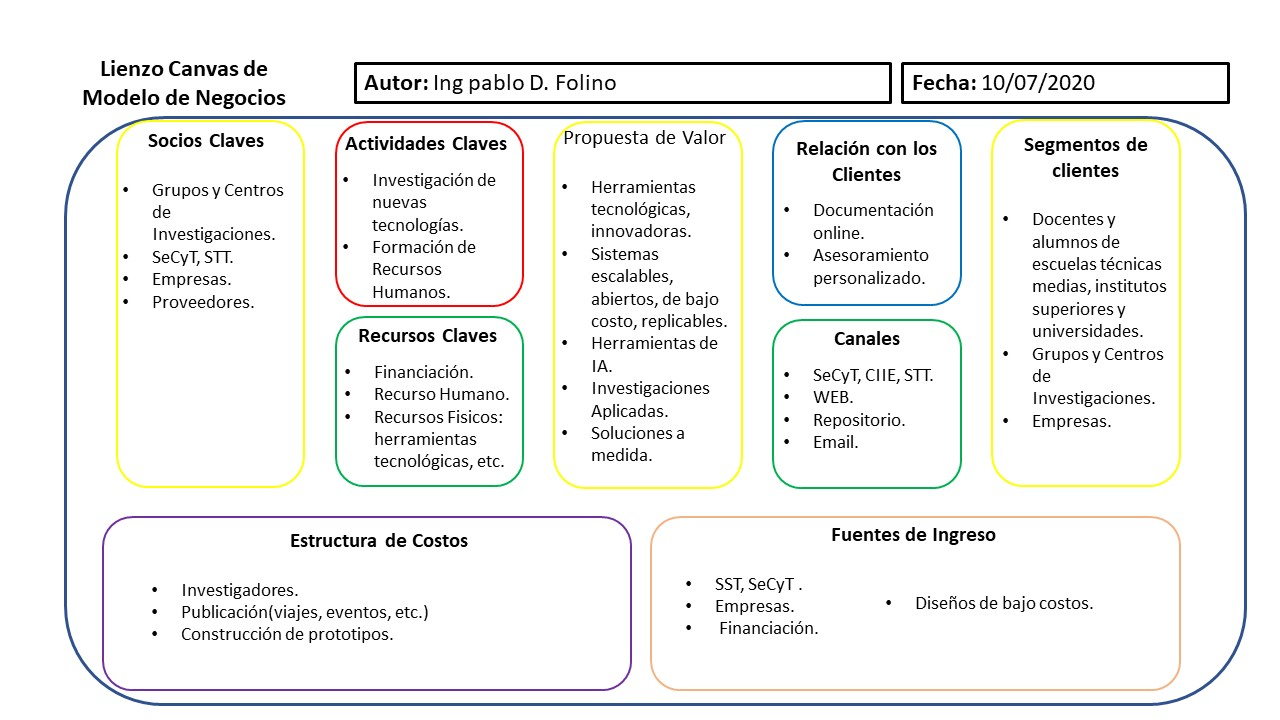
\includegraphics[width=\textwidth]{./Figuras/GIAR.jpg}
\caption{Diagrama modelo de negocios \textit{GIAR}}
\label{fig:ModNegGIAR}
\end{figure}


Se pretende diseñar un Sistema Embebido para desplazar un pequeño robot de 20x15x10 cm (aprox.) traccionado por dos motores de corriente contínua en configuración triciclo, con  un módulo GPS, y conexión WIFI, como se observa en la figura \ref{fig:diagConceptual}. 

%La descripción técnica-conceptual \textbf{debe incluir al menos un diagrama en bloques del sistema }y una frase como la siguiente: ``En la Figura \ref{fig:diagBloques} se presenta el diagrama en bloques del sistema. Se observa que...''. Luego recién más abajo de haber puesto esta frase se pone la figura. La regla es que las figuras nunca pueden ir antes de ser mencionadas en el texto, porque sino el lector no entiende por qué de pronto aparece una figura.

\vspace{25px}

\begin{figure}[htpb]
\centering 
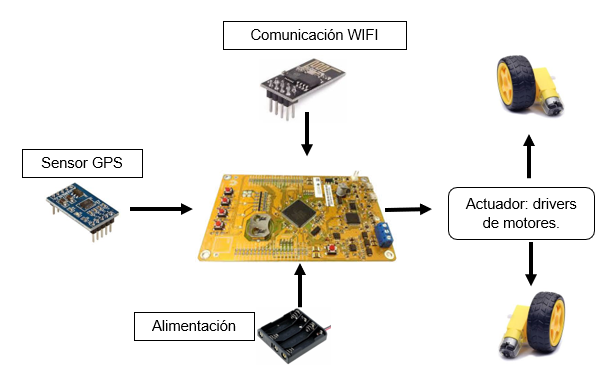
\includegraphics[width=.8\textwidth]{./Figuras/Robot.png}
\caption{Diagrama conceptual del sistema}
\label{fig:diagConceptual}
\end{figure}

\vspace{25px}

El cerebro del sistema será una placa EDU-CIAA-NPX, que recibirá la información de los distintos sensores y controlará los actuadores. Los motores serán controlados por un puente H (driver) mediante pulsos de PWM (modulación de ancho de pulso). La placa recibirá información de comunicación por un módulo WIFI (del tipo ESP8266), y de un módulo GPS. En lo posible, también se instalará un acelerómetro para usarlo en la lógica del algoritmo de AR.
El sistema será alimentado por un \textit{pack} de baterías, que serán seleccionadas en función del consumo/autonomía y peso del robot.
Además, para poder comparar el sistema de control embebido en la placa principal, se instalará un control PID (Proporcional, Integral y Derivativo), sintonizado a las condiciones estándares de funcionamiento del sistema.
El robot estará diseñado para moverse en espacios interiores (\textit{indoor}), en un suelo plano y liso, en condiciones de temperaturas estándares entre 5 ºC y 40 ºC, y humedad relativa normales(entre 40 \% y 70 \%). 


%El tamaño de la tipografía en la figura debe ser adecuado para que NO pase lo que ocurre acá, donde el lector debe esforzarse para poder leer el texto. Los colores usados en el diagrama deben ser adecuados, tal que ayuden a comprender mejor el diagrama.
%\end{consigna}


\section{Identificación y análisis de los interesados}
\label{sec:interesados}

%\begin{consigna}{red} 
%Nota: (borrar esto y todas las consignas en color rojo antes de entregar este documento).
 
%Es inusual que una misma persona esté en más de un rol, incluso en proyectos chicos.
 
%Si se considera que una persona cumple dos o más roles, entonces sólo dejarla en el rol más importante. Por ejemplo:
%\begin{itemize}
%\item Si una persona es Cliente pero también colabora u orienta, dejarla solo como Cliente.
%\item Si una persona es el Responsable, no debe ser colocado también como Miembro del equipo.
%\end{itemize}
%Pero en cambio sí es usual que el Cliente y el Auspiciante sean el mismo, por ejemplo.

\begin{table}[ht]
%\caption{Identificación de los interesados}
%\label{tab:interesados}
\begin{tabularx}{\linewidth}{@{}|l|X|X|l|@{}}
\hline
\rowcolor[HTML]{C0A0C0} 
Rol           & Nombre y Apellido & Organización 	& Puesto 	\\ \hline
%Auspiciante   & -  				& -					& -	   		\\ \hline
Cliente       & \clientename    &\empclientename	& -   		\\ \hline
Impulsor      & Secretario de SeCyT    		&\empclientename 	& -   		\\ \hline
Responsable   & \authorname     & FIUBA        		& Alumno 	\\ \hline
Colaboradores & Miembros del GIAR   & UTN-FRBA     		& -       	\\ \hline
Orientador    & \supname	    & \pertesupname 	& Director	trabajo final \\ \hline
%Equipo        & -          		& -             	& -        	\\ \hline
Opositores    & Otros Grupos Invest.    & UTN-FRBA             	& -        	\\ \hline
Usuario final & Alumnos de materia -IA     &\empclientename	& -        	\\ \hline
\end{tabularx}
\end{table}

%El Director suele ser uno de los Orientadores.
%No dejar celdas vacías; si no hay nada que poner en una celda colocar un signo ``-''.
%No dejar filas vacías; si no hay nada que poner en una fila entonces eliminarla.

%Sería deseable listar a continuación de la tabla las principales características de cada interesado.
 
%Por ejemplo:
%\begin{itemize}
%\item Auspiciante: es riguroso y exigente con la rendición de gastos. Tener mucho cuidado con esto.
%\item Equipo: Juan Perez, suele pedir licencia porque tiene un familiar con una enfermedad. Planificar considerando esto.
%\item Orientador: María Gómez, nos va a poder ayudar mucho con la gestión de impuestos.
%\end{itemize}

%\end{consigna}

\begin{itemize}
\item Orientador: Ing. Juan Carlos Gómez, posee mucha experiencia en el tema debido a su trabajo, y formación  profesional, pero no posee mucho tiempo.
\item Cliente: posee muchas restricciones con respecto a los costos.
\end{itemize}

\section{1. Propósito del proyecto}
\label{sec:proposito}

%\begin{consigna}{red}
%¿Por qué se hace el proyecto? ¿Qué se quiere lograr? 
%\end{consigna}

El propósito de este proyecto es desarrollar y probar  algoritmos de AR para poder mover un robot, y aplicar los conocimientos en materias de Inteligencia Artificial  dictadas en la UTN-FRBA.



\section{2. Alcance del proyecto}
\label{sec:alcance}

%\begin{consigna}{red}
%¿Qué se incluye y que no se incluye en este proyecto?
%Se refiere al trabajo a hacer para entregar el producto o resultado especificado. 
%Explicitar todo lo quede comprendido dentro del alcance del proyecto.
%Explicitar además todo lo que no quede incluido (``El presente proyecto no incluye...'')
%\end{consigna}
 
El objetivo del proyecto comprende:

\begin{itemize}
\item Diseñar y armar el prototipo del hardware del robot, tipo triciclo.
\item Diseñar e implementar en la placa EDU-CIAA-NXP el software embebido de A.R.
\item Diseñar comandos para cambiar el modo de funcionaniento desde línea de comandos, desde una PC. 
\item Realizar el proyecto dentro del tiempo destinado al mismo.
\end{itemize}

El proyecto no incluye:

\begin{itemize}
\item Realizar pruebas de estructuras de hardware, para saber la vida útil del sistema.
\item Diseñar una interface gráfica amigable para cambiar los distintos modos de funcionamiento.
\item Diseñar y/o armar el cargador de baterías.
\item Carcasa, ni gabinete para el robot.
\end{itemize}


\section{3. Supuestos del proyecto}
\label{sec:supuestos}

%\begin{consigna}{red}
%``Para el desarrollo del presente proyecto se supone que: ...''

Se supone para el siguiente proyecto que:
\begin{itemize}
\item se posee el presupuesto para comprar todo lo relacionado con el hardware necesario para construir el robot. 
\item se contará con acceso a todo el equipamiento para la construcción y testeo de los distintos elementos electrónicos.
\item la complejidad de la programación se restringirá en función de las horas de trabajo propuestas para hacer este proyecto.
\item se podrá conseguir los distintos elementos electrónicos en este contexto de pandemia.
\end{itemize}

%Por ejemplo, se podrían incluir supuestos respecto a disponibilidad de tiempo y recursos humanos y materiales, sobre la factibilidad técnica de distintos aspectos del proyecto, sobre otras cuestiones que sean necesarias para el éxito del proyecto como condiciones macroeconómicas o reglamentarias.
%\end{consigna}

\section{4. Requerimientos}
\label{sec:requerimientos}

%\begin{consigna}{red}
%Los requerimientos deben numerarse y de ser posible agruparlos por afinidad:

\begin{enumerate}
\item Requerimientos de funcionamiento general
	\begin{enumerate}
	\item El sistema debe tener una autonomía de por lo menos 10 minutos.
	\item Se debe comunicar en forma inalámbrica. 
	\item Debe ser un robot pequeño de dimensiones(no mayor a 25x20x15 cm).
	\item Debe ser un robot liviano (no mayor a 1,25 Kg)
	\end{enumerate}
\item Grupo de requerimientos asociados con el hardware
	\begin{enumerate}
	\item El hardware debe ser fácilmente replicable, utilizando una impresora 3D.
	\item Debe poseer la menor cantidad de piezas posibles, no mayor a diez. 
	\item El cuerpo del robot debe albergar todo el hardware (motores, placa EDU-CIAA, drivers de motores, baterías, etc.) necesario para el funcionamiento normal.
	\item Debe poseer un botón de parada de emergencia de fácil acceso, para interrumpir el funcionamiento del robot en caso de urgencia.
	\end{enumerate}
\item Grupo de requerimientos asociados con el software
	\begin{enumerate}
	\item Se programará usando Lenguaje C, utilizando el modelo de capas y las sAPI del proyecto CIAA.
	\item La herramienta de programación en Lenguaje C deberá poseer un modo DEBUG.
	\item El uso de memoria no debe exceder a la placa EDU-CIAA-NXP.
	\end{enumerate}
\item Requerimientos no funcionales
	\begin{enumerate}
	\item La estructura del robot no debe tener bordes filosos ni punzantes, que puedan ocasionar lesiones. 
	\item La velocidad que desarrolla el robot debe ser inferior a 1 m/seg.
	\end{enumerate}
\item Requerimientos documentación
	\begin{enumerate}
	\item Redactar el manual de uso. 
	\item Redactar un documento en donde se registre el código 
	fuente.
	\item Redactar un documento técnico que figuren los circuitos
	esquemáticos, y el armado de la plataforma.
	\end{enumerate}
\end{enumerate}

%Leyendo los requerimientos se debe poder interpretar cómo será el proyecto y su funcionalidad.
%De ser posible indicar cómo se obtuvieron cada uno de los requerimientos 
%Indicar claramente cuál es la prioridad entre los distintos requerimientos. 

%No olvidarse de que los requerimientos incluyen a las regulaciones y normas vigentes!!!

%Y al escribirlos seguir las siguientes reglas:
%\begin{itemize}
%\item Ser breve y conciso (nadie lee cosas largas). 
%\item Ser específico: no dejar lugar a confusiones.
%\item Expresar los requerimientos en términos que sean cuantificables y medibles.
%\end{itemize}

%\end{consigna}


\section{Historias de usuarios (\textit{Product backlog})}
\label{sec:backlog}

\begin{consigna}{red}
Descripción: En esta sección se deben incluir las historias de usuarios y su ponderación (\textit{history points}). Recordar que las historias de usuarios son descripciones cortas y simples de una característica contada desde la perspectiva de la persona que desea la nueva capacidad, generalmente un usuario o cliente del sistema. La ponderación es un número entero que representa el tamaño de la historia comparada con otras historias de similar tipo.
\end{consigna}

\vspace{40mm}


\section{5. Entregables principales del proyecto}
\label{sec:entregables}

%\begin{consigna}{red}
Al final del proyecto se entregará: 
\begin{itemize}
\item Prototipo del robot.
\item Manual de uso.
\item Diagrama esquemático.
\item Código fuente.
\item Diagrama de instalación.
\item Informe final.

\end{itemize}

%\end{consigna}

\section{6. Desglose del trabajo en tareas}
\label{sec:wbs}
%\begin{consigna}{red}
%Se recomienda mostrar el WBS mediante una lista indexada:
\begin{enumerate}
\item Planificación de tareas. (40 hs)
	\begin{enumerate}
	\item Generación del documento de planificación del proyecto. (30 hs)
	\item Aprobación y revisión del documento de planificación del proyecto. (10 hs)
	\end{enumerate}
\item Investigación preliminar del hardware a utilizar. (38 hs)
	\begin{enumerate}
	\item Fabricación del robot. (20 hs)
	\item Placas electrónicas(placa principal, microcontrolador, drivers, etc). (10 hs)
	\item Características de los motores.  (4 hs)
	\item Características de las baterías. (4 hs)
	\end{enumerate}
\item Selección y compra de los materiales del hardware. (8 hs)
	\begin{enumerate}
	\item Selección de los componentes. (5 hs)
	\item Compra y adquisición.(3 hs)
	\end{enumerate}
\item Armado y verificación de la estructura del robot. (28 hs)
	\begin{enumerate}
	\item Construcción de las piezas. (15 hs)
	\item Ensamblaje de piezas. (3 hs)
	\item Verificación de la estructura. (10 hs)
	\end{enumerate}
\item Armado y verificación de la electrónica del robot. (10 hs)
	\begin{enumerate}
	\item Armado de la placa adaptadora entre EDU-CIAA y los distintos módulos. (5 hs)
	\item Cableado del robot. (2 hs)
	\item Verificación de la electrónica. (3 hs)
	\end{enumerate}	
\item Integración del hardware. (2 hs)	
\item Desarrollo del software (240 hs)
	\begin{enumerate}
	\item Módulo PWM. (25 hs)
	\item Módulo WIFI y protocolo de comunicaciones. (40 hs)
	\item Módulo GPS. (25 hs)
	\item Módulo acelerómetro.  (25 hs)
	\item Sensores de fines de carrera. (30 hs)
	\item Módulo de aprendizaje por refuerzo. (40 hs)
	\item Módulo PID. (25 hs)
	\item Integración de los distintos módulos. (30 hs)
	\end{enumerate}	
\item Verificación del software(\textit{Testing}). (75 hs)
	\begin{enumerate}
	\item Diseño de pruebas  de ensayo de los distintos módulos. (25 hs)
	\item Diseño de las distintas pruebas de navegación. (30 hs)
	\item Comparación de las distintas estrategias de navegación. (20 hs)
	\end{enumerate}	
\item Validación del sistema completo. (40 hs)
	\begin{enumerate}
	\item Ensayos de verificación del cliente en forma parcial. (20 hs)
	\item Ensayos de validación final. (20 hs)
	\end{enumerate}	
\item Presentación del trabajo. (151 hs)
	\begin{enumerate}
	\item Redacción de informes de avance. (10 hs)
	\item Redacción de manual de uso. (20 hs)
	\item Elaboración de circuitos esquemáticos. (20 hs)
	\item Redacción de memoria del proyecto. (80 hs)
	\item Preparación de la presentación pública del trabajo final. (20 hs)
	\item Presentación pública del trabajo final. (1 h)
	\end{enumerate}					
\end{enumerate}
Cantidad total de horas: (632 hs)
%Se recomienda que no haya ninguna tarea que lleve más de 40 hs. 
%\end{consigna}

\vspace{80mm}

\section{7. Diagrama de Activity On Node}
\label{sec:AoN}
En la figura \ref{fig:AoN}, se observa el camino crítico en color rojo. Las unidades de tiempo definida en cada tarea es en horas reloj. 
\begin{figure}[htpb]
\centering 
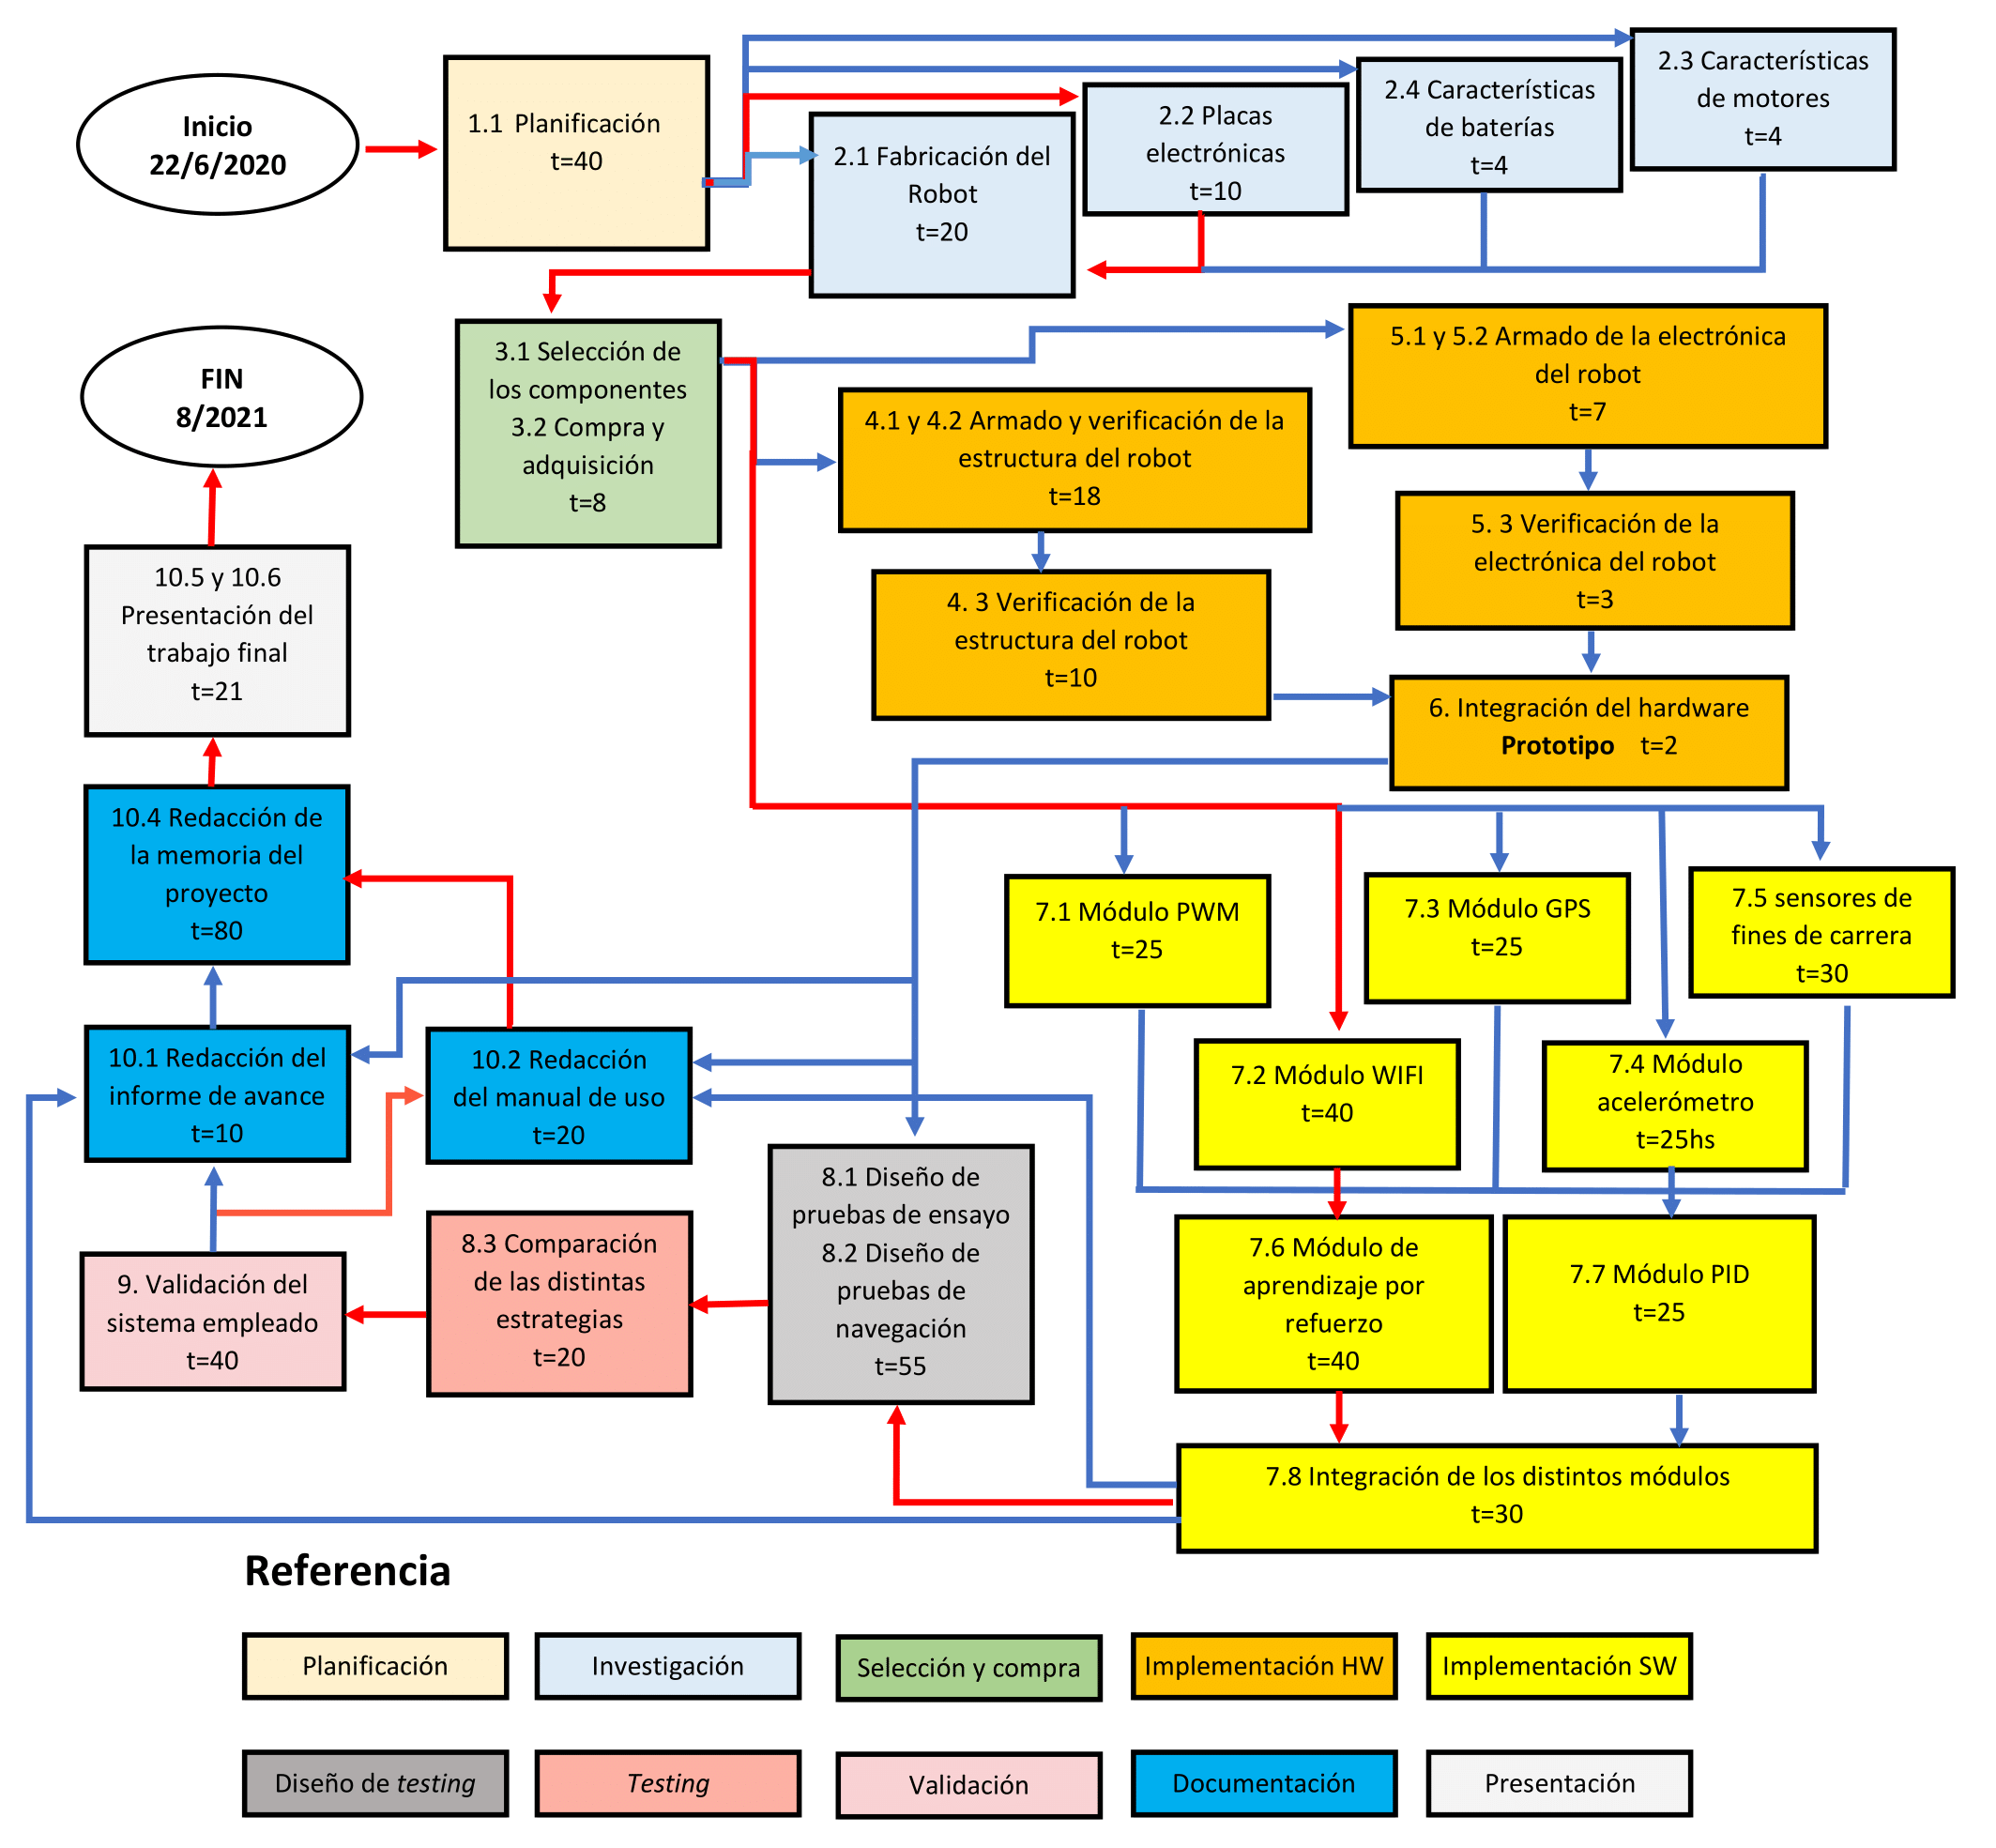
\includegraphics[width=.8\textwidth]{./Figuras/AoN.png}
\caption{Diagrama de \textit{Activity on Node}}
\label{fig:AoN}
\end{figure}

\vspace{80mm}


\section{8. Diagrama de Gantt}
\label{sec:gantt}
\begin{table}[htbp]
\centering
\resizebox{0.95\textwidth}{!}{
\begin{tabular}{|p{25em}|c|c|c|}
\hline
\textbf{Nombre de tarea} & \textbf{Duración} & \textbf{Comienzo}& \textbf{Fin} \\
\hline  \textbf{Inicio} & 0 días & lun 22/6/20 & lun 22/6/20 \\
\hline \textbf{1. Planificación de tareas} & \textbf{20 días} & textbf{lun 22/6/20} & textbf{mar 21/7/20} \\
\hline 1.1 Generación de documento & 30 horas & lun 22/6/20 & mar 14/7/20 \\
\hline 1.2 Aprobación y revisión & 10 horas & mié 15/7/20 &  mar 21/7/20 \\
\hline \textbf{2. Investigación preliminar del hardware} & \textbf{12 días} & \textbf{mié 22/7/20} & \textbf{jue 6/8/20} \\
\hline 2.1 Fabricación del Robot & 20 horas & \ mié 22/7/20 & jue 6/8/20 \\
\hline 2.2 Placas electrónicas & 10 horas & mié 22/7/20 & mar 28/7/20 \\
\hline 2.3 Características de motores & 4 horas & mié 29/7/20 & jue 30/7/20 \\
\hline 2.4 Características de baterías & 4 horas & vie 31/7/20 & lun 3/8/20 \\
\hline \textbf{3. Selección y compra de los materiales} & \textbf{4 días} & \textbf{vie 7/8/20} & \textbf{mié 12/8/20} \\
\hline 3.1 Selección de los componentes & 5 horas & vie 7/8/20 & mar 11/8/20 \\
\hline 3.2 Compra y adquisición & 3 horas & mar 11/8/20 & mié 12/8/20 \\
\hline textbf{4. Armado y verificación de la estructura del robot} & \textbf{14 días} & \textbf{jue 13/8/20} & \textbf{mié 2/9/20} \\
\hline 4.1 Construcción de las piezas & 15 horas & jue 13/8/20 & mar 25/8/20 \\
\hline 4.2 Ensamblaje de las piezas & 3 horas & mar 25/8/20 & mié 26/8/20 \\
\hline 4.3 Verificación de la estructura & 10 horas & jue 27/8/20 & mié 2/9/20 \\
\hline \textbf{5. Armado y verificación de la electrónica del robot} & \textbf{5 días} & \textbf{jue 3/9/20} & \textbf{mié 9/9/20} \\
\hline 5.1 Armado de la EDU-CIAA & 5 horas & jue 3/9/20 & lun 7/9/20 \\
\hline 5.2 Cableado del robot & 2 horas & lun 7/9/20 & mar 8/9/20 \\
\hline 5.3 Verificación de la electrónica & 3 horas & mar 8/9/20 & mié 9/9/20 \\
\hline 6. Integración del hardware & 2 horas & jue 10/9/20 & jue 10/9/20 \\
\hline \textbf{7. Desarrollo del software} & \textbf{87,5 días} & \textbf{vie 11/9/20} & \textbf{jue 21/1/21} \\
\hline 7.1 Módulo PWM & 25 horas & vie 11/9/20 & mar 29/9/20 \\
\hline 7.2 Módulo WIFI & 40 horas & vie 11/9/20 & jue 8/10/20 \\
\hline 7.3 Módulo GPS & 25 horas & mar 29/9/20 & vie 16/10/20 \\
\hline 7.4 Módulo acelerómetro & 25 horas & vie 9/10/20 & mié 28/10/20 \\
\hline 7.5 sensores de fines de carrera & 30 horas & lun 19/10/20 & vie 6/11/20 \\
\hline 7.6 Módulo de aprendizaje por refuerzo & 40 horas & jue 26/11/20 & mar 29/12/20 \\
\hline 7.7 Módulo PID & 25 horas & lun 9/11/20 & jue 26/11/20 \\
\hline 7.8 Integración de los distintos módulos & 30 horas & mar 29/12/20 & jue 21/1/21 \\
\hline \textbf{8. Verificación del software} & \textbf{37,5 días} & \textbf{jue 21/1/21} & \textbf{lun 15/3/21} \\
\hline 8.1 Diseño de pruebas de ensayo & 25 horas & jue 21/1/21 & lun 8/2/21 \\
\hline 8.2 Diseño de pruebas de navegación & 30 horas & mar 9/2/21 & lun 1/3/21 \\
\hline 8.3 Comparación de las distintas estrategias. & 20 horas & mar 2/3/21 & lun 15/3/21 \\
\hline textbf{9. Validación del sistema empleado} & \textbf{20 días} & \textbf{mar 16/3/21} & \textbf{mié 14/4/21} \\
\hline 9.1 Ensayos de verificación del cliente parcial & 20 horas & mar 16/3/21 & mar 30/3/21 \\
\hline9.2 Ensayos de validación final & 20 horas & mié 31/3/21 & mié 14/4/21 \\
\hline \textbf{10. Presentación del trabajo final} & \textbf{75,5 días} & \textbf{jue 15/4/21} & \textbf{lun 2/8/21} \\
\hline 10.1 Redacción del informe de avance & 10 horas & jue 15/4/21 & mié 21/4/21 \\
\hline 10.2 Redacción del manual de uso & 20 horas & jue 22/4/21 & mié 5/5/21 \\
\hline 10.3 Elaboración de los circuitos esquemáticos & 20 horas & jue 6/5/21 & mié 19/5/21 \\
\hline 10.4 Redacción de la memoria del proyecto & 80 horas & jue 20/5/21 & vie 16/7/21 \\
\hline 10.5 Preparación de la presentación pública & 20 horas & lun 19/7/21 & vie 30/7/21 \\
\hline 10.6 Presentación pública & 1 hora & lun 2/8/21 & lun 2/8/21 \\
\hline FIN   & 0 días & lun 2/8/21 & lun 2/8/21 \\
\hline
\end{tabular}}
\caption{\textit{Gantt}}
\label{tab:CuadroGantt}
\end{table}

Los datos de la cuadro \ref{tab:CuadroGantt} y de la figura \ref{fig:Gantt} se obtuvieron de un software de gestión de proyectos teniendo en cuenta los días no laborables, y con una dedicación semanal de 10 horas reloj.  

%\begin{consigna}{red}
%Utilizar el software Gantter for Google Drive o alguno similar para %dibujar el diagrama de Gantt.
%Existen muchos programas y recursos \textit{online} para hacer %diagramas de gantt, entre las cuales destacamos:

%\begin{itemize}
%\item Planner
%\item GanttProject
%\item Trello + \textit{plugins}. En el siguiente link hay un %tutorial oficial: \\ \url{https://blog.trello.com/es/diagrama-de-%gantt-de-un-proyecto}
%\item Creately, herramienta online colaborativa. \\\url{https://%creately.com/diagram/example/ieb3p3ml/LaTeX}
%\item Se puede hacer en latex con el paquete \textit{pgfgantt}\\ %\url{http://ctan.dcc.uchile.cl/graphics/pgf/contrib/pgfgantt/%pgfgantt.pdf}
%\end{itemize}

%Pegar acá una captura de pantalla del diagrama de Gantt, cuidando %que la letra sea suficientemente grande como para ser legible. 
%Si el diagrama queda demasiado ancho, se puede pegar primero la %``tabla'' del Gantt y luego pegar la parte del diagrama de barras %del diagrama de Gantt.

%Configurar el software para que en la parte de la tabla muestre los %códigos del EDT (WBS).\\
%Configurar el software para que al lado de cada barra muestre el %nombre de cada tarea.\\
%Revisar que la fecha de finalización coincida con lo indicado en el %Acta Constitutiva.

%En la figura \ref{fig:gantt}, se muestra un ejemplo de diagrama de %gantt realizado con el paquete de \textit{pgfgantt}. En la %plantilla pueden ver el código que lo genera y usarlo de base para %construir el propio.

%\begin{figure}[htbp]
%\begin{center}
%\begin{ganttchart}{1}{12}
%  \gantttitle{2020}{12} \\
%  \gantttitlelist{1,...,12}{1} \\
%  \ganttgroup{Group 1}{1}{7} \\
%  \ganttbar{Task 1}{1}{2} \\
%  \ganttlinkedbar{Task 2}{3}{7} \ganttnewline
%  \ganttmilestone{Milestone o hito}{7} \ganttnewline
%  \ganttbar{Final Task}{8}{12}
%  \ganttlink{elem2}{elem3}
%  \ganttlink{elem3}{elem4}
%\end{ganttchart}
%\end{center}
%\caption{Diagrama de gantt de ejemplo}
%\label{fig:gantt}
%\end{figure}

%\end{consigna}
\newpage
\begin{landscape}
\begin{figure}[htpb]
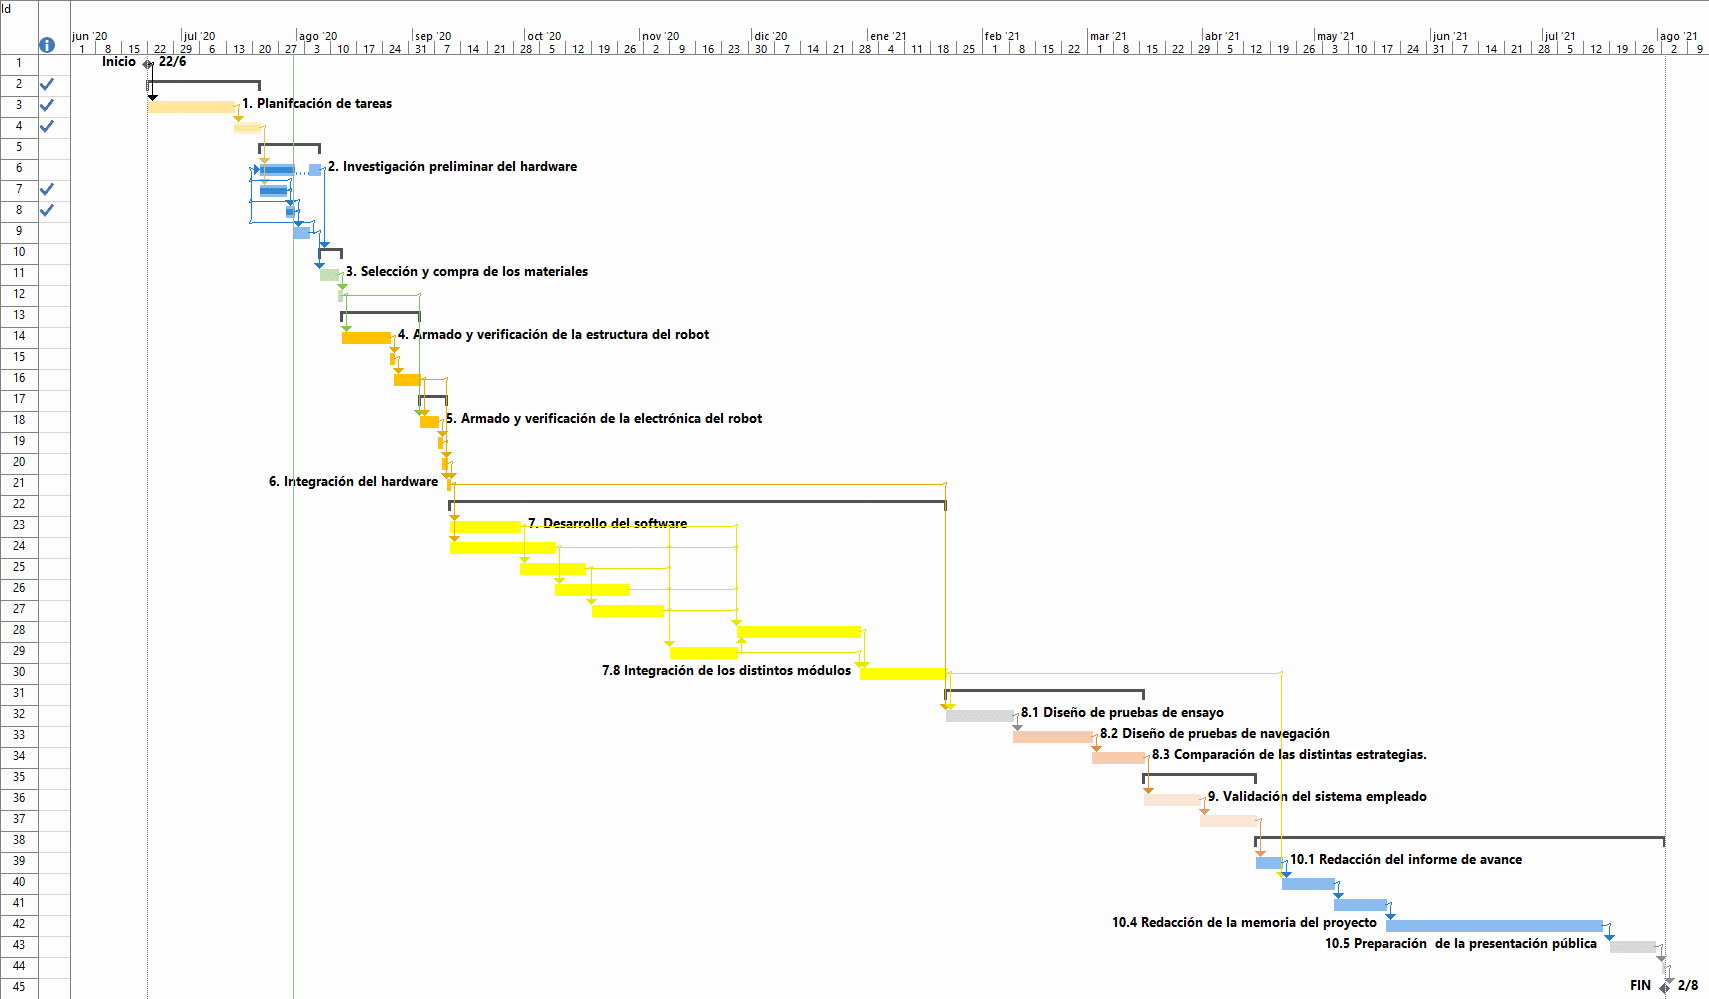
\includegraphics[width=1.6\textwidth]{./Figuras/Gantt.png}
\caption{Diagrama de \textit{Gantt}}
\label{fig:Gantt}
\end{figure}
\end{landscape}



\section{9. Matriz de uso de recursos de materiales}
\label{sec:recursos}


\begin{table}[htpb] 
\label{tab:recursos}
\centering
%\scalebox{1.1}[1.2]{}
\begin{tabularx}{\linewidth}{@{}|p{1.5em}|X|c|c|c|c|c|c|@{}} 
\hline
\multicolumn{1}{|c|}{\cellcolor[HTML]{C0A0C0}} & \multicolumn{1}{|c|}{\cellcolor[HTML]{C0A0C0}} & \multicolumn{6}{|c|}{\cellcolor[HTML]{C0A0C0}Recursos requeridos (horas)}\\ \cline{3-8} 
\multicolumn{1}{|c|}{\rotatebox{90} {\cellcolor[HTML]{C0A0C0} ~~Nº Tarea}}
& \multicolumn{1}{|c|}{\multirow{-6}{*}{\cellcolor[HTML]{C0A0C0} Nombre de la tarea}}

& \rotatebox{75} {\cellcolor[HTML]{A0A0C0} PC-Internet}
 
& \rotatebox{75} {\cellcolor[HTML]{A0A0A0}Impresora-3D} 

& \rotatebox{75} {\cellcolor[HTML]{A0A0C0} Comp.elect.} 

& \rotatebox{75} {\cellcolor[HTML]{A0B0B0} Tester } 

&  \rotatebox{75} {\cellcolor[HTML]{A0A0C0} Oscilosc.} 

&  \rotatebox{75} {\cellcolor[HTML]{B0B0B0} Filmadora  } 

\\ \hline

1.& Planificación & \cellcolor[HTML]{A0A0C0}20&\cellcolor[HTML]{A0A0A0}& \cellcolor[HTML]{A0A0C0}&\cellcolor[HTML]{A0B0B0}&
\cellcolor[HTML]{A0A0C0}&\cellcolor[HTML]{B0B0B0}
\\ \hline

2.& Investigación  & \cellcolor[HTML]{A0A0C0}20&\cellcolor[HTML]{A0A0A0}20& \cellcolor[HTML]{A0A0C0}&\cellcolor[HTML]{A0B0B0}1&
\cellcolor[HTML]{A0A0C0}&\cellcolor[HTML]{B0B0B0}
\\ \hline

3.&Selección y Compra & \cellcolor[HTML]{A0A0C0}2&\cellcolor[HTML]{A0A0A0}& \cellcolor[HTML]{A0A0C0}5&\cellcolor[HTML]{A0B0B0}&
\cellcolor[HTML]{A0A0C0}&\cellcolor[HTML]{B0B0B0}
\\ \hline

4.& Armado de la estruc.del robot  & \cellcolor[HTML]{A0A0C0}20&\cellcolor[HTML]{A0A0A0}15& \cellcolor[HTML]{A0A0C0}5&\cellcolor[HTML]{A0B0B0}1&
\cellcolor[HTML]{A0A0C0}&\cellcolor[HTML]{B0B0B0}1
\\ \hline

5.& Armado de placas electrónicas  & \cellcolor[HTML]{A0A0C0}5&\cellcolor[HTML]{A0A0A0}& \cellcolor[HTML]{A0A0C0}10&\cellcolor[HTML]{A0B0B0}10&
\cellcolor[HTML]{A0A0C0}2&\cellcolor[HTML]{B0B0B0}
\\ \hline

6.& Armado HW & \cellcolor[HTML]{A0A0C0}&\cellcolor[HTML]{A0A0A0}& \cellcolor[HTML]{A0A0C0}1&\cellcolor[HTML]{A0B0B0}1&
\cellcolor[HTML]{A0A0C0}&\cellcolor[HTML]{B0B0B0}0,5
\\ \hline

7.& Diseño del SW  & \cellcolor[HTML]{A0A0C0}200&\cellcolor[HTML]{A0A0A0}& \cellcolor[HTML]{A0A0C0}10&\cellcolor[HTML]{A0B0B0}&
\cellcolor[HTML]{A0A0C0}&\cellcolor[HTML]{B0B0B0}
\\ \hline

8.& Verificación(\textit{testing})& \cellcolor[HTML]{A0A0C0}60&\cellcolor[HTML]{A0A0A0}& \cellcolor[HTML]{A0A0C0}10&\cellcolor[HTML]{A0B0B0}1&
\cellcolor[HTML]{A0A0C0}&\cellcolor[HTML]{B0B0B0}0,5
\\ \hline

9.& Validación  & \cellcolor[HTML]{A0A0C0}30&\cellcolor[HTML]{A0A0A0}& \cellcolor[HTML]{A0A0C0}40&\cellcolor[HTML]{A0B0B0}&
\cellcolor[HTML]{A0A0C0}&\cellcolor[HTML]{B0B0B0}1
\\ \hline

10.& Presentación Documentación  & \cellcolor[HTML]{A0A0C0}120&\cellcolor[HTML]{A0A0A0}& \cellcolor[HTML]{A0A0C0}20&\cellcolor[HTML]{A0B0B0}&
\cellcolor[HTML]{A0A0C0}&\cellcolor[HTML]{B0B0B0}5
\\ \hline
\end{tabularx}
\end{table}

\vspace{40em}


\section{10. Presupuesto detallado del proyecto}
\label{sec:presupuesto}

%\begin{consigna}{red}
%Si el proyecto es complejo entonces separarlo en partes:
%\begin{itemize}
%\item Un total global, indicando el subtotal acumulado por cada una de las áreas.
%\item El desglose detallado del subtotal de cada una de las áreas.
%\end{itemize}

%IMPORTANTE: No olvidarse de considerar los COSTOS INDIRECTOS.

%\end{consigna}
\begin{table}[htpb]
\centering
\begin{tabularx}{\linewidth}{@{}|p{1em}|X|X|X|X|@{}}
\hline
\rowcolor[HTML]{C0C0C0} 
\multicolumn{5}{|c|}{\cellcolor[HTML]{C0A0C0}COSTOS DIRECTOS [\$]} \\ \hline
\rowcolor[HTML]{C0C0C0} 
\multicolumn{2}{|c|}{Descripción} &
  \multicolumn{1}{c|}{\cellcolor[HTML]{B0B0B0}Cantidad} &
  \multicolumn{1}{c|}{\cellcolor[HTML]{B0B0B0}Valor unitario} &
  \multicolumn{1}{c|}{\cellcolor[HTML]{B0B0B0}Valor total} \\ \cline{1-5}
\multirow{13}[1]{*}{\rotatebox{90}{Materiales}} & Driver doble puente H  (L298) &
  \multicolumn{1}{c|}{1} &
  \multicolumn{1}{c|}{550} &
  \multicolumn{1}{c|}{550} \\ \cline{2-5}
& Motor CC con reducción  5v&
   \multicolumn{1}{c|}{2} &
  \multicolumn{1}{c|}{310} &
  \multicolumn{1}{c|}{620} \\ \cline{2-5}
& Placa EDU-CIAA-NXP &
   \multicolumn{1}{c|}{1} &
  \multicolumn{1}{c|}{6.500} &
  \multicolumn{1}{c|}{6.500} \\ \cline{2-5}
& Porta baterías (4 pilas AA) &
  \multicolumn{1}{c|}{1} &
  \multicolumn{1}{c|}{1} &
  \multicolumn{1}{c|}{290} \\ \cline{2-5}
&  Baterias de Li-ion 1500 mah&
   \multicolumn{1}{c|}{4} &
  \multicolumn{1}{c|}{250} &
  \multicolumn{1}{c|}{1.000} \\ \cline{2-5}
& Pulsador NA &
  \multicolumn{1}{c|}{1} &
  \multicolumn{1}{c|}{100} &
  \multicolumn{1}{c|}{100} \\ \cline{2-5}
& Placa  WIFI(ESP1 8266)&
   \multicolumn{1}{c|}{1} &
  \multicolumn{1}{c|}{500} &
  \multicolumn{1}{c|}{500} \\ \cline{2-5} 
&  Placa acelerómetro (Mpu-9250)&
   \multicolumn{1}{c|}{1} &
  \multicolumn{1}{c|}{790} &
  \multicolumn{1}{c|}{790} \\ \cline{2-5}
&  Cables varios &
  \multicolumn{1}{c|}{1} &
  \multicolumn{1}{c|}{1} &
  \multicolumn{1}{c|}{260} \\ \cline{2-5}
&  Conectores varios &
  \multicolumn{1}{c|}{1} &
  \multicolumn{1}{c|}{1} &
  \multicolumn{1}{c|}{560} \\ \cline{2-5}
&  Placa experimental 10x10 cm &
  \multicolumn{1}{c|}{1} &
  \multicolumn{1}{c|}{350} &
  \multicolumn{1}{c|}{350} \\ \cline{2-5}
&  Estaño 60/40 0,8mm 3m&
  \multicolumn{1}{c|}{1} &
  \multicolumn{1}{c|}{250} &
  \multicolumn{1}{c|}{250} \\ \cline{2-5} 
&  Filamento 1.75mm (PLA) &
  \multicolumn{1}{c|}{1} &
  \multicolumn{1}{c|}{1.000} &
  \multicolumn{1}{c|}{1000} \\ \cline{2-5}    
&  Ruedas &
  \multicolumn{1}{c|}{2} &
  \multicolumn{1}{c|}{130} &
  \multicolumn{1}{c|}{260} \\ \cline{1-5} 
\multicolumn{4}{|c|}{Mano de obra} &
  \multicolumn{1}{c|}{150.000} \\ \hline
  
\multicolumn{4}{|c|}{SUBTOTAL} &
  \multicolumn{1}{c|}{163.030} \\ \hline
\rowcolor[HTML]{C0C0C0} 
\multicolumn{5}{|c|}{\cellcolor[HTML]{C0A0C0}COSTOS INDIRECTOS [\$]} \\ \hline
\rowcolor[HTML]{C0C0C0} 
\multicolumn{4}{|c|}{Descripción} &
  \multicolumn{1}{c|}{\cellcolor[HTML]{B0B0B0}Valor total} \\ \hline
\multicolumn{4}{|c|}{30\% de los costos directos} &
  \multicolumn{1}{c|}{48.909} \\ \hline
  
\multicolumn{4}{|c|}{SUBTOTAL [\$]} &
  \multicolumn{1}{c|}{48.909} \\ \hline
\multicolumn{4}{|c|}{\cellcolor[HTML]{B0B0B0}TOTAL [\$]} &
  \multicolumn{1}{c|}{\cellcolor[HTML]{B0B0B0}211.939} \\ \hline   
\end{tabularx}
\caption{Presupuesto}
\label{tab:Presupuesto}
\end{table}


Aclaración: el presupuesto de la cuadro \ref{tab:Presupuesto} se realizó con fecha 25/07/2020 con una cotización del dólar estadounidense de \$120.

\vspace{40em}

\section{11. Matriz de asignación de responsabilidades}
\label{sec:responsabilidades}
\renewcommand{\tabularxcolumn}[1]{>{\arraybackslash}m{#1}}
\begin{table}[htbp]
\centering
%\resizebox{.9\textwidth}{!}{
\begin{tabularx}{\textwidth}{@{}|c|p{11em}|p{5.8em}|p{4.8em}|p{6em}|X|@{}}
\hline
\cellcolor[HTML]{C0A0C0}\begin{tabular}{cc} \rotatebox{90}{Nº} &   \rotatebox{90}{Tarea} \end{tabular} 
&
\cellcolor[HTML]{C0A0C0}\begin{tabular}{ccc} & \rotatebox{45}{Nombre de la tarea}& \end{tabular} 
&
\cellcolor[HTML]{C0A0C0}\begin{tabular}{rc} \rotatebox{90}{\textbf{Responsable}} & \rotatebox{90}{\authorname} \end{tabular} 
&
\cellcolor[HTML]{C0A0C0}\begin{tabular}{rc} \rotatebox{90}{\textbf{Director}} & \rotatebox{90}{\supname} \end{tabular} 
& 
\cellcolor[HTML]{C0A0C0}\begin{tabular}{rc} \rotatebox{90}{\textbf{Cliente}} & \rotatebox{90}{\clientename} \end{tabular}  
& 
\cellcolor[HTML]{C0A0C0}\begin{tabular}{c} \rotatebox{90}{} \\ \rotatebox{90}{\textbf{~~Jurado}} \end{tabular} \\

\hline \rowcolor[gray]{.8}
1.1 & Generación Documentación & \multicolumn{1}{c|}{P} & \multicolumn{1}{c|}{C} & &  \\
\hline 
1.2 & Aprobación y revisión del documento &\multicolumn{1}{c|}{P} &\multicolumn{1}{c|}{A}& \multicolumn{1}{c|}{A} &\multicolumn{1}{c|}{I} \\
\hline \rowcolor[gray]{.8}
2. & Investigación HW &\multicolumn{1}{c|}{P} & \multicolumn{1}{c|}{C} &   &  \\
\hline
3. & Selección y compra &\multicolumn{1}{c|}{P} &\multicolumn{1}{c|}{I} &\multicolumn{1}{c|}{A} &  \\
\hline \rowcolor[gray]{.8}
4., 5.y 6. & Armado del HW &\multicolumn{1}{c|}{P} &\multicolumn{1}{c|}{I}  &   &  \\
\hline
7. & Desarrollo del SW &\multicolumn{1}{c|}{P} &\multicolumn{1}{c|}{C} & & \\
\hline \rowcolor[gray]{.8}
8. & \textit{Testing} &\multicolumn{1}{c|}{P} &\multicolumn{1}{c|}{S} &\multicolumn{1}{c|}{I} &\multicolumn{1}{c|}{I}\\
\hline
9. &  Validación &\multicolumn{1}{c|}{P} &\multicolumn{1}{c|}{A} &\multicolumn{1}{c|}{A} &\multicolumn{1}{c|}{I} \\
\hline \rowcolor[gray]{.8}
10.1 & Redacción informe &\multicolumn{1}{c|}{P} &\multicolumn{1}{c|}{A} &  &\multicolumn{1}{c|}{I} \\
\hline
10.2 & Redacción del manual &\multicolumn{1}{c|}{P} &\multicolumn{1}{c|}{A} &   &  \\
\hline \rowcolor[gray]{.8}
10.3 & Elaboración de circuitos esquemáticos &\multicolumn{1}{c|}{P} &  \multicolumn{1}{c|}{I} &   & \\
\hline
10.4 & Redacción de la memoria &\multicolumn{1}{c|}{P}  &\multicolumn{1}{c|}{A} &   &\multicolumn{1}{c|}{I} \\
\hline \rowcolor[gray]{.8}
10.5 & Preparación de la presentación &\multicolumn{1}{c|}{P}  &\multicolumn{1}{c|}{A} &  &\multicolumn{1}{c|}{I} \\
\hline
10.6 & Presentación pública &\multicolumn{1}{c|}{P} &\multicolumn{1}{c|}{I} &  & \multicolumn{1}{c|}{A} \\
\hline 
\end{tabularx}%}
\caption{Matriz de asignaciones de responsabilidades}
\label{tab:addlabel}
\end{table}

{\footnotesize
Referencias:
\begin{itemize}
	\item P = Responsabilidad Primaria
	\item S = Responsabilidad Secundaria
	\item A = Aprobación
	\item I = Informado
	\item C = Consultado
\end{itemize}
} %footnotesize


%\begin{consigna}{red}
%Establecer la matriz de asignación de responsabilidades y el manejo %de la autoridad completando la siguiente tabla:

%\begin{table}[htpb]
%\centering
%\resizebox{\textwidth}{!}{
%\begin{tabular}{|c|c|c|c|c|c|}
%\hline \rowcolor[HTML]{C0C0C0} \cellcolor[HTML]{C0C0C0} &
%  \cellcolor[HTML]{C0C0C0} &\multicolumn{4}{c|}{\cellcolor[HTML]{C0C0C0} Listar todos los nombres y roles del proyecto} \\ \cline{3-6} 
%\rowcolor[HTML]{C0C0C0} 
%\cellcolor[HTML]{C0C0C0} &
%  \cellcolor[HTML]{C0C0C0} &
%  Responsable &
%  Orientador &
%  Equipo &
%  Cliente \\ \cline{3-6} 
%\rowcolor[HTML]{C0C0C0} 
%\multirow{-3}{*}{\cellcolor[HTML]{C0C0C0}\begin{tabular}[c]{@{}c@{}}Código\\ WBS\end{tabular}} &
%  \multirow{-3}{*}{\cellcolor[HTML]{C0C0C0}Nombre de la tarea} &
%  \authorname &
%  \supname &
%  Nombre de alguien &
%  \clientename \\ \hline
% &  &  &  &  &  \\ \hline
% &  &  &  &  &  \\ \hline
% &  &  &  &  &  \\ \hline
%\end{tabular}%
%}
%\end{table}



%Una de las columnas debe ser para el Director, ya que se supone que %participará en el proyecto.
%A su vez se debe cuidar que no queden muchas tareas seguidas sin %``A'' o ``I''.

%Importante: es redundante poner ``I/A'' o ``I/C'', porque para aprobarlo o responder consultas primero la persona debe ser informada.

%\end{consigna}


\vspace{40em}

\section{12. Gestión de riesgos}
\label{sec:riesgos}

a) Identificación de los riesgos: 
\renewcommand{\tabularxcolumn}[1]{>{\arraybackslash}m{#1}}
\begin{table}[htpb]
\centering
\resizebox{.97\textwidth}{!}{
\begin{tabularx}{\textwidth}{@{}|c|p{3em}|m{4em}|c|X|@{}}
\hline
\multicolumn{1}{|c|}{\cellcolor[HTML]{C0A0C0}Nro.} &
\multicolumn{1}{|c|}{\cellcolor[HTML]{C0A0C0}Descripción del riesgo} &
\multicolumn{1}{|c|}{\cellcolor[HTML]{C0A0C0}\begin{tabular}{m{4em}}Severidad \\ Ocurrencia \end{tabular} } &
\multicolumn{1}{|c|}{\cellcolor[HTML]{C0A0C0}Valor}&
\multicolumn{1}{|c|}{\cellcolor[HTML]{C0A0C0} Justificación}\\ \hline

\multirow{2}{*}{1}  							&
	\multirow{2}{*}{\begin{tabular}{c}
	Pérdida/Destrucción \\
	del kit de desarrollo \end{tabular}}		&
	Severidad 									&
	10											&
	EL daño en el kit de desarrollo impacta en 
	numerosas etapas del desarrollo de este 
	proyecto.  \\ \cline{3-5}
	& &
	Ocurrencia 									&
	5											&
	La posibilidad que esto suceda es moderada, ya 
	que el kit se montará en una plataforma móvil.
	\\ \hline
\multirow{2}{*}{2}  							&
	\multirow{2}{*}{\begin{tabular}{c}
	Destrucción del \\
	driver de motor \\
	(L298) \end{tabular}}		&
	Severidad 									&
	7											&
	EL daño en el driver atrasaría algunas tareas,
	pero otras  podrían continuar.  \\ \cline{3-5}
	& &
	Ocurrencia 									&
	6											&
	Si el motor se bloquea, por el driver puede 
	circular mucha corriente y se puede quemar.
	\\ \hline

\multirow{2}{*}{3}  							&
	\multirow{2}{*}{\begin{tabular}{c}
	Falta de tiempo  \\
	para adquirir los \\
	conocimientos \\
	para implementar el \\software de	AR. 
	\end{tabular}}								&
	Severidad 									&
	6											&
	El algoritmo se está probando en otra plataforma
	pero de características muy distintas.  \\ \cline{3-5}
	& &
	Ocurrencia 									&
	3											&
	La probabilidad es baja, ya que se puede adaptar
	distintos niveles de complejidad.
	\\ \hline

\multirow{2}{*}{4}  							&
	\multirow{2}{*}{\begin{tabular}{c}
	Daños en la \\ 
	impresora 3D.  \end{tabular}}				&
	Severidad 									&
	6											&
	Se usa para fabricar las piezas del robot en
	un etapa temprana el proyecto. \\ \cline{3-5}
	& &
	Ocurrencia 									&
	7											&
	La probabilidad es alta, ya que su funcionamiento depende
	de muchos factores (que los inyectores no se tapen, que las
	tensiones de las correas sean las correctas, que no se
	quemen los drivers de los motores, que el firmware
	no se dañe, etc ).	\\ \hline
	
\multirow{2}{*}{5}  							&
	\multirow{2}{*}{\begin{tabular}{c}
	Capacidad o poten-\\
	cia  del pack de bate-\\
	ría insuficiente para\\
	cumplir con los reque-\\
	rimientos planteados\\
	\end{tabular}}								&
	Severidad 									&
	6											&
	Se usan baterías Li-ion, algunos consumos pueden
	ser vitales para el éxito del proyecto. \\ \cline{3-5}
	& &
	Ocurrencia 									&
	7											&
	La probabilidad es alta, no se tiene experiencia en el 
	manejo de este tipo de batería.	\\ \hline	
	
\multirow{2}{*}{6}  							&
	\multirow{2}{*}{\begin{tabular}{c}
	Daño en la computa-\\ 
	dora que se usa para \\
 	programar y docu- \\
	mentar el proyecto.
	\end{tabular}}								&
	Severidad 									&
	7											&
	Se usa para el diseño de las piezas del robot,
	programar los algoritmos en la placa EDU-CIAA,
	y la documentación del proyecto. \\ \cline{3-5}
	& &
	Ocurrencia 									&
	5											&
	No es una computadora moderna, su probabilidad de falla es 
	considerable.	\\ \hline	
	
\end{tabularx}
}
\caption{Gestión de riesgos}
\label{tab:GestionRiesgos}
\end{table}

La ``severidad'' y la ``probabilidad de ocurrencia'' se califican de 1 a 10, siendo el número más alto correspondiente a la mayor severidad o la mayor probabilidad.
\vspace{5em}

%\begin{consigna}{red}
%a) Identificación de los riesgos (al menos cinco) y estimación %de sus consecuencias: 
%Riesgo 1: detallar el riesgo (riesgo es algo que si ocurre %altera los planes previstos)
%\begin{itemize}
%\item Severidad (S): mientras más severo, más alto es el número %(usar números del 1 al 10).\\
%Justificar el motivo por el cual se asigna determinado número de %severidad (S).
%\item Probabilidad de ocurrencia (O): mientras más probable, más %alto es el número (usar del 1 al 10).\\
%Justificar el motivo por el cual se asigna determinado número de %(O). 
%\end{itemize}   

%Riesgo 2:
%\begin{itemize}
%\item Severidad (S): 
%\item Ocurrencia (O):
%\end{itemize}

%Riesgo 3:
%\begin{itemize}
%\item Severidad (S): 
%\item Ocurrencia (O):
%\end{itemize}

b) Tabla de gestión de riesgos: (El RPN se calcula como \%RPN=SxO)

\begin{table}[htpb]
\centering
\begin{tabular}{@{}|c|c|c|c|c|c|c|@{}}
\hline
\rowcolor[HTML]{C0C0C0} 
\cellcolor[HTML]{C0A0C0}Nº de Riesgo & \cellcolor[HTML]{C0A0C0}S & \cellcolor[HTML]{C0A0C0}O & \cellcolor[HTML]{C0A0C0}RPN & \cellcolor[HTML]{C0A0C0}S* & \cellcolor[HTML]{C0A0C0}O* & \cellcolor[HTML]{C0A0C0}RPN* \\ \hline
 1	& 10 & 5 & \cellcolor{red} 50 & 5 & 5 & \cellcolor{green}25     \\ \hline
 2	&  7 & 6 & \cellcolor{red}42 & 3 & 5 & \cellcolor{green}15     \\ \hline
 3	&  6 & 3 & \cellcolor{green}18 &    &    &      \\ \hline
 4	&  6 & 7 & \cellcolor{red}42 & 6 & 3 & \cellcolor{green}18     \\ \hline
 5  &  6 & 7 & \cellcolor{red}42 & 3 & 5 & \cellcolor{green}15     \\ \hline
 6  &  7 & 5 & \cellcolor{green}35 &    &    &      \\ \hline
\end{tabular}%
\caption{RPN}
\label{tab:RPN}
\end{table}

\textbf{Criterio adoptado}: se tomarán medidas de mitigación de los riesgos cuyos RPN sean mayores a 40.

\textbf{Aclaración}: en la tabla \ref{tab:RPN} los valores marcados con (*) corresponden luego de haber aplicado el plan de mitigación de riesgos.

%\begin{consigna}{red}
%b) Tabla de gestión de riesgos:      (El RPN se calcula como %RPN=SxO)

%\begin{table}[htpb]
%\centering
%\begin{tabularx}{\linewidth}{@{}|X|c|c|c|c|c|c|@{}}
%\hline
%\rowcolor[HTML]{C0C0C0} 
%Riesgo & S & O & RPN & S* & O* & RPN* \\ \hline
%       &   &   &     &    &    &      \\ \hline
%       &   &   &     &    &    &      \\ \hline
%       &   &   &     &    &    &      \\ \hline
%       &   &   &     &    &    &      \\ \hline
%       &   &   &     &    &    &      \\ \hline
%\end{tabularx}%
%\end{table}

%Criterio adoptado: 
%Se tomarán medidas de mitigación en los riesgos cuyos números de %RPN sean mayores a ....

%Nota: los valores marcados con (*) en la tabla corresponden %luego de haber aplicado la mitigación.


c) Plan de mitigación de los riesgos que originalmente excedían el RPN máximo establecido:
 
\begin{itemize}
\item Riesgo 1: Pérdida/Destrucción	del kit de desarrollo.
	Medidas de mitigación: Para minimizar este riesgo se prevee un apartida presupuestaria para comprar otra placa en caso de que sea necesario. Se habla con el proveedor y asegura tener \textit{stock} para los próximos meses y un plazo de entrega no mayor a 24 horas.
	\begin{itemize}
	\item Severidad(S): 5 Disminuye la severidad, algunas tareas pueden tener un retraso no significativo. 
	\item  Probabilidad de ocurrencia(O): 5 La probabilidad de ocurrencia no cambia debido al escaso conocimiento de la placa EDU-CIAA-NPX. 
	\end{itemize}
\item Riesgo 2:  Falta de tiempo para adquirir los conocimientos
para implementar el software de AR.
	Medidas de mitigación: El firmware de la placa en un primer prototipo puede salir con una versión acotada, al proyecto estaría aprobado por el cliente con el módulo del PID clásico y una de las técnicas de aprendizaje por refuerzo. Se puede recurrir al asesoramiento de expertos en el tema.
	\begin{itemize}
	\item Severidad(S): 3 La severidad disminuye considerablemente, se tiene la posibilidad de tener otras fuentes de información.
	\item  Probabilidad de ocurrencia(O): 5 Probabilidad de ocurrencia media, hay que ver la disponibilidad de los horarios de los expertos en el tema para ver si pueden atender nuestras consultas.  
	\end{itemize} 
\item Riesgo 4: Daños en la	impresora 3D.
	Medidas de mitigación: Se debe tener en \textit{stock} los repuestos necesarios para reemplazar en caso de ser necesarios. Los repuestos como la boquilla fusora, y las correas dentadas no son caras y se consiguen en el mercado.
	\begin{itemize}
	\item Severidad(S): 6 La severidad no cambia, la impresión de las piezas es un punto critico.
	\item  Probabilidad de ocurrencia(O): 3 Disminuye considerablemente, ya que al tener los repuestos se puede prevenir que no deje de funcionar. Hay algunos repuestos como la placa de control que son difíciles de conseguir, en tal caso hay que recurrir a otro tipo de estrategia de mitigación
	\end{itemize}
\item Riesgo 5: Capacidad o potencia del pack de batería	insuficiente para cumplir con los requerimientos planteados.
	Medidas de mitigación: Se debe diseñar el pack de batería para tener la posibilidad o de ampliar la capacidad de \textit{mAh} de las baterías de \textit{Li-ion}, o cambiarlas por otra tecnología como de \textit{NiCd} o \textit{NiMH}. Por tal motivo en el diseño se adoptó el uso de baterías de formato AA o 14500.
	\begin{itemize}
	\item Severidad(S): 3 Disminuye considerablemente al tener varias alternativas.
	\item  Probabilidad de ocurrencia(O): 5 La probabilidad de ocurrencia es media, ya que de algunas baterías se carece del conocimiento de funcionamiento detallado. 
	\end{itemize}
\end{itemize}



%Riesgo 1: Plan de mitigación (si por el RPN fuera necesario %elaborar un plan de mitigación).
%  Nueva asignación de S y O, con su respectiva justificación:
%  - Severidad (S): mientras más severo, más alto es el número (usar %números del 1 al 10).
%          Justificar el motivo por el cual se asigna determinado %número de severidad (S).
%  - Probabilidad de ocurrencia (O): mientras más probable, más alto %es el número (usar del 1 al 10).
%          Justificar el motivo por el cual se asigna determinado %número de (O).

%Riesgo 2: Plan de mitigación (si por el RPN fuera necesario elaborar un plan de mitigación).
 
%Riesgo 3: Plan de mitigación (si por el RPN fuera necesario %elaborar un plan de mitigación)

%\end{consigna}


\section{13. Gestión de la calidad}
\label{sec:calidad}

%------------------------------------------------------------------
%\begin{consigna}{red}
%Para cada uno de los requerimientos del proyecto indique:
%\begin{itemize} 
%\item Req \#1: Copiar acá el requerimiento.

%Verificación y validación:

%\begin{itemize}
%\item Verificación para confirmar si se cumplió con lo requerido %antes de mostrar el sistema al cliente:\\
%Detallar 
%\item Validación con el cliente para confirmar que está de acuerdo %en que se cumplió con lo requerido:\\
%Detallar  
%\end{itemize}

%\end{itemize}

%Tener en cuenta que en este contexto se pueden mencionar %simulaciones, cálculos, revisión de hojas de datos, consulta con %expertos, etc.
%\end{consigna}
%----------------------------------------------------------%\renewcommand\labelitemi{$\clubsuit$}

1. Requerimientos de funcionamiento general.
\begin{itemize} 
\item Req \#1.1: El sistema debe tener una autonomía de por lo menos 10 minutos. 
\begin{itemize}
\item Verificación y validación:
	\begin{itemize}
	\item Verificación para confirmar si se cumplió con lo requerido 	antes de mostrar el sistema al cliente:\\
	Se verifican los consumos de todas las placas del sistema 				mediante las hojas de datos y mediciones empíricas. Se hacen los 	cálculos de consumos y se registra la autonomía del robot en 			condiciones normales de funcionamiento. Con la batería al 100\%
	 de carga, se hace mover al robot en distintas direcciones y se
	 registra en cuánto tiempo tarda hasta que no pueda responder a
	  los comandos enviados.
	\item Validación con el cliente para confirmar que está de 				acuerdo en que se cumplió con lo requerido:\\
	Con la baterìa completa se hará mover al robot en círculos, en 			una superficie plana durante el lapso de 10 minutos para validad 	este requerimiento.
	\end{itemize}
\end{itemize}	
\end{itemize}

\begin{itemize} 
\item Req \#1.2: Se debe comunicar en forma inalámbrica.
\begin{itemize} 
\item Verificación y validación:
	\begin{itemize}
	\item Verificación para confirmar si se cumplió con lo requerido 	antes de mostrar el sistema al cliente:\\
	Se verificarán las hojas de datos del módulo inalámbrico, 
	distancia de comunicación, velocidad de comunicación, potencia
	de transmisión, etc. Se verificarán si se hace el	
	\textit{``chequeo de verificación de trama''} mandando tramas no
	validas o con errores de secuencia, el robot la descarte.
	\item Validación con el cliente para confirmar que está de 				acuerdo en que se cumplió con lo requerido:\\
	Mediante una prueba empírica se le envía comandos de movimiento
	al robot (hacia adelante, hacia atrás, giro a la derecha e
	izquierda), para demostrar que la plataforma móvil responde.
\end{itemize}
	
	\end{itemize}
\end{itemize}

\begin{itemize} 
\item Req \#1.3: Debe ser un robot pequeño de dimensiones(no mayor a 25x20x15 cm).
\begin{itemize} 
\item Verificación y validación:
	\begin{itemize}
	\item Verificación para confirmar si se cumplió con lo requerido 	antes de mostrar el sistema al cliente:\\
	Se realiza las mediciones del robot.  
	\item Validación con el cliente para confirmar que está de 				acuerdo en que se cumplió con lo requerido:\\
	Mediante un cubo de dimensiones de 25x25x15 cm con uno de los
	lados de la base abierta, se hace entrar al robot para validar
	este requerimiento.  
	\end{itemize}
\end{itemize}
\end{itemize}

\begin{itemize}
\item Req \#1.4: Debe ser un robot liviano (no mayor a 1,25 Kg).
\begin{itemize} 
\item Verificación y validación:
	\begin{itemize}
	\item Verificación para confirmar si se cumplió con lo requerido 	antes de mostrar el sistema al cliente:\\
	Mediante las hojas de datos o en forma práctica, se elaborará un
	documento en donde se registren los pesos de cada componente. Se
	verificará que la suma total de los componentes no supere los
	1,25 Kg.
	\item Validación con el cliente para confirmar que está de 				acuerdo en que se cumplió con lo requerido:\\
	Mediante una balanza se pesa la plataforma móvil para validar
	este requerimiento.  
	\end{itemize}
\end{itemize}
\end{itemize}

2. Grupo de requerimientos asociados con el hardware.

\begin{itemize}
\item Req \#2.1: El hardware debe ser fácilmente replicable, utilizando una impresora 3D.
\begin{itemize}
\item Verificación y validación:
	\begin{itemize}
	\item Verificación para confirmar si se cumplió con lo requerido 	antes de mostrar el sistema al cliente:\\
	Se verifican que todos los elementos estructurales del
 	robot puedan realizarse por una impresora 3D con un solo 
 	extrusor, eso significa que no se necesite por ejemplo de
 	material de soporte	especiales, que las dimensiones sean
 	menores que una cama de impresión estándar (20x20 cm), 
 	que el filamento sea fácil de conseguir (PLA o ABS), etc.
	\item Validación con el cliente para confirmar que está de 				acuerdo en que se cumplió con lo requerido:\\
	Se muestran los planos de donde se obtuvieron las impresiones de 
	los componentes  que conforman la plataforma.    
	\end{itemize}
\end{itemize}
\end{itemize}

\begin{itemize}
\item Req \#2.2: Debe poseer la menor cantidad de piezas posibles, no mayor a diez. utilizando una impresora 3D.
\begin{itemize}
\item Verificación y validación:
	\begin{itemize}
	\item Verificación para confirmar si se cumplió con lo requerido 	antes de mostrar el sistema al cliente:\\
	Se hace un listado detallado de todos los componentes
	estructurales del hardware y se verifican que la cantidad sea 
	menor a la del requerimiento.
	\item Validación con el cliente para confirmar que está de 				acuerdo en que se cumplió con lo requerido:\\
	Se muestra al cliente el listado detallado elaborado en la
	 prueba de verificación. 
	\end{itemize}
\end{itemize}
\end{itemize}

\begin{itemize}
\item Req \#2.3: El cuerpo del robot debe albergar todo el hardware (motores, placa EDU-CIAA, drivers de motores, baterías, etc.) necesario para el funcionamiento normal.
\begin{itemize}
\item Verificación y validación:
	\begin{itemize}
	\item Verificación para confirmar si se cumplió con lo requerido 	antes de mostrar el sistema al cliente:\\
	Mediante planos se verifica que todos los elementos
	estructurales del robot, las distintas placas, los motores, y
	sensores se encuentran autocontenidos.  
	\item Validación con el cliente para confirmar que está de 				acuerdo en que se cumplió con lo requerido:\\
	Se demuestra al cliente empíricamente se cumple este requisito.
	\end{itemize}
\end{itemize}
\end{itemize}

\begin{itemize}
\item Req \#2.4: Debe poseer un botón de parada de emergencia de fácil acceso, para interrumpir el funcionamiento del robot en caso de urgencia.
\begin{itemize}
\item Verificación y validación:
	\begin{itemize}
	\item Verificación para confirmar si se cumplió con lo requerido 	antes de mostrar el sistema al cliente:\\
	Se depura el programa  y verifica que sin importar en que
	secuencia de programa se encuentre el software, al pulsar el
	botón se invoca la rutina de parada.  
	\item Validación con el cliente para confirmar que está de 				acuerdo en que se cumplió con lo requerido:\\
	Se hace funcionar al robot en una  trayectoria circular, y se
	verifica que cuando se presiona el botón de parada cumple este
	requerimiento.  
	\end{itemize}
\end{itemize}
\end{itemize}

3. Grupo de requerimientos asociados con el software.

\begin{itemize}
\item Req \#3.1: Se programará usando Lenguaje C, utilizando el modelo de capas y las sAPI del proyecto CIAA.
\begin{itemize}
\item Verificación y validación:
	\begin{itemize}
	\item Verificación para confirmar si se cumplió con lo requerido 	antes de mostrar el sistema al cliente:\\
	Se analizarán las hojas de datos de la placa EDU-CIAA  y se
	verificará que usando un ambiente de programación en Lenguaje C
	se pueda programar la placa. Se controlará que todo el código
	fuente utilizado para programar al producto final esté escrito
	en Lenguaje C y con llamadas a las sAPI.
	Se generará un documento en donde se registren todas las rutinas
	que conforman el proyecto. 
	\item Validación con el cliente para confirmar que está de 				acuerdo en que se cumplió con lo requerido:\\
	Se presentará el informe del listado del código fuente con las
	rutinas que conforman el proyecto.   
	\end{itemize}
\end{itemize}
\end{itemize}

\begin{itemize}
\item Req \#3.2: La herramienta de programación en Lenguaje C deberá poseer un modo DEBUG.
\begin{itemize}
\item Verificación y validación:
	\begin{itemize}
	\item Verificación para confirmar si se cumplió con lo requerido 	antes de mostrar el sistema al cliente:\\
	Se verificará de las hojas de datos de la placa de desarrollo
	que posea un puerto serie extra, o algún otro método que permita tener información de depuración. 
	\item Validación con el cliente para confirmar que está de 				acuerdo en que se cumplió con lo requerido:\\
	Se configurará el prototipo para que envíe información de depuración a través de algún medio de comunicación con el cliente.
	\end{itemize}
\end{itemize}
\end{itemize}

\begin{itemize}
\item Req \#3.3: El uso de memoria no debe exceder a la placa EDU-CIAA-NXP.
\begin{itemize}
\item Verificación y validación:
	\begin{itemize}
	\item Verificación para confirmar si se cumplió con lo requerido 	antes de mostrar el sistema al cliente:\\
	Se analizará las hojas de datos de la placa de control y de su
	microprocesador para que con el código generado en el proyecto cumpla con este requerimiento.
	\item Validación con el cliente para confirmar que está de 				acuerdo en que se cumplió con lo requerido:\\
	Se compilará y  un programa de prueba en la placa de
 	desarrollo para validar el requerimiento.
	\end{itemize}
\end{itemize}
\end{itemize}

4. Requerimientos no funcionales

\begin{itemize}
\item Req \#4.1: La estructura del robot no debe tener bordes filosos ni punzantes, que puedan ocasionar lesiones. 
\begin{itemize}
\item Verificación y validación:
	\begin{itemize}
	\item Verificación para confirmar si se cumplió con lo requerido 	antes de mostrar el sistema al cliente:\\
	Se verificará con los planos estructurales de las piezas del
	robot, que todos los bordes externos si terminan en una arista,
	no sean ángulos inferiores a 90 grados, o que sean redondeados
	con un diámetro mayor a 0,5 mm. Se generará un informe
	detallando.
	\item Validación con el cliente para confirmar que está de 				acuerdo en que se cumplió con lo requerido:\\
	Se presentará el informe generado en la validación, constatando  
	físicamente con el robot.
	\end{itemize}
\end{itemize}
\end{itemize}

\begin{itemize}
\item Req \#4.2: La velocidad que desarrolla el robot debe ser inferior a 1 m/seg. 
\begin{itemize}
\item Verificación y validación:
	\begin{itemize}
	\item Verificación para confirmar si se cumplió con lo requerido 	antes de mostrar el sistema al cliente:\\
 	Con las hojas de datos del motor (máxima \textit{rpm}) y el
 	diámetro de la rueda se calculará la velocidad máxima del robot.
	\item Validación con el cliente para confirmar que está de 				acuerdo en que se cumplió con lo requerido:\\
	Se medirá la velocidad que alcanza el robot a máxima carga de
	batería con un método indirecto. Se pondrán a 5 metros de
	distancia en línea recta dos marcas en un piso plano y liso. El
	robot se pondrá en posición de reposo a un metro atrás de la
	primera marca y se acelerará a máxima velocidad. Se medirá el
	tiempo en que tarda en cruzar las dos marcas, calculando así su
	velocidad máxima.   
	\end{itemize}
\end{itemize}
\end{itemize}


5. Requerimientos de documentación

\begin{itemize}
\item Req \#5.1: Redactar manual de uso. 
\begin{itemize}
\item Verificación y validación:
	\begin{itemize}
	\item Verificación para confirmar si se cumplió con lo requerido 	antes de mostrar el sistema al cliente:\\
	Se irá controlando la generación parcial de este documento
	técnico.
	\item Validación con el cliente para confirmar que está de 				acuerdo en que se cumplió con lo requerido:\\
	El director del proyecto validará este documento.  
	\end{itemize}
\end{itemize}
\end{itemize}

\begin{itemize}
\item Req \#5.2: Redactar un documento en donde se registre el código fuente. 
\begin{itemize}
\item Verificación y validación:
	\begin{itemize}
	\item Verificación para confirmar si se cumplió con lo requerido 	antes de mostrar el sistema al cliente:\\
	Se irá controlando la generación parcial de documentación
	técnica, para que sirva de referencia para la posterior
	escritura de la memoria.
	\item Validación con el cliente para confirmar que está de 				acuerdo en que se cumplió con lo requerido:\\
	El director y los jurados leerán esta información en la memoria
	técnica y la validarán.
	\end{itemize}
\end{itemize}
\end{itemize}

\begin{itemize}
\item Req \#5.3: Redactar un documento técnico que figuren los circuitos esquemáticos, y el armado de la plataforma.
\begin{itemize}
\item Verificación y validación:
	\begin{itemize}
	\item Verificación para confirmar si se cumplió con lo requerido 	antes de mostrar el sistema al cliente:\\
	Se irá controlando la generación parcial de documentación
	técnica, para que sirva de referencia para la posterior
	escritura de la memoria.
	\item Validación con el cliente para confirmar que está de 				acuerdo en que se cumplió con lo requerido:\\
	El director y los jurados leerán esta información en la memoria
	técnica y la validarán.   
	\end{itemize}
\end{itemize}
\end{itemize}

%\vspace{1mm}
\clearpage

\section{14. Comunicación del proyecto}
\label{sec:comunicaciones}

%\begin{consigna}{red}
%El plan de comunicación del proyecto es el siguiente:
%\end{consigna}

% Please add the following required packages to your document preamble:
% \usepackage{graphicx}
% \usepackage[table,xcdraw]{xcolor}
% If you use beamer only pass "xcolor=table" option, i.e. \documentclass[xcolor=table]{beamer}

\renewcommand{\tabularxcolumn}[1]{>{\arraybackslash}m{#1}}
\begin{table}[htpb]
\centering
\resizebox{\textwidth}{!}{%
\begin{tabularx}{\textwidth}{@{}|X|X|X|X|X|X|@{}}
\hline
\rowcolor[HTML]{C0C0C0} 
\multicolumn{6}{|c|}{\cellcolor[HTML]{C0A0C0}Plan de comunicación del proyecto}           \\ \hline
\rowcolor[HTML]{C0A0C0} 
¿Qué comunicar? & Audiencia & Propósito & Frecuencia & Método de comunicac. & Responsable \\ \hline
Definición de los objetivos y los alcances &
Director &  Evaluación & Inicio del proyecto & Correo electrónico                     &\authorname          \\ \hline
                
Inicio de las tareas de implementación &
Director  &  Informar & Inicio de implementación  &   Correo electrónico                    
&\authorname         \\ \hline
                
Grado de avance & Director & Informar y evaluar & Al término de cada tarea &  Correo electrónico &\authorname         \\ \hline
                
Problemas que puedan afectar los tiempos de entrega &  Director Cliente & Informar & Cuando surjan  & Correo electrónico                      &\authorname        \\ \hline
                
Finalización y cierre &  Director   Jurados & Evaluación & Final del proyecto &  Correo electrónico   	
&\authorname     \\ \hline
\end{tabularx}
}
\end{table}

\vspace{20mm}

\section{15. Gestión de Compras}
\label{sec:compras}

%\begin{consigna}{red}
%En caso de tener que comprar elementos o contratar servicios:
%a) Explique con qué criterios elegiría a un proveedor.
%b) Redacte el Statement of Work correspondiente.
%\end{consigna}
\underline{Criterio de selección de proveedores:}

Tanto para la compra de componentes electrónicos  como de filamentos PLA para la confección del robot, se seleccionarán aquellos proveedores del mercado nacional que dispongan de \textit{stock} suficiente de los componentes requeridos, presenten una cotización menor, entreguen a domicilio, y que los tiempos de entrega sean dentro de las 24 hrs. Dado que los componentes a utilizar pueden ser adquiridos por varios proveedores, se descarta un análisis de los mismos.

\vspace{200mm}

\section{16. Seguimiento y control}
\label{sec:seguimiento}

%\begin{consigna}{red}
%Para cada tarea del proyecto establecer la frecuencia y los indicadores con los se seguirá su avance y quién será el responsable de hacer dicho seguimiento y a quién debe comunicarse la situación (en concordancia con el Plan de Comunicación del proyecto).
%
%El indicador de avance tiene que ser algo medible, mejor incluso si se puede medir en \% de avance. Por ejemplo,se pueden indicar en esta columna cosas como ``cantidad de conexiones ruteadeas'' o ``cantidad de funciones implementadas'', pero no algo genérico y ambiguo como ``\%'', porque el lector no sabe porcentaje de qué cosa.
%
%\end{consigna}
%
%\begin{table}[!htpb]
%\centering
%\begin{tabularx}{\linewidth}{@{}|X|X|X|X|X|X|@{}}
%\hline
%\rowcolor[HTML]{C0C0C0} 
%\multicolumn{6}{|c|}{\cellcolor[HTML]{C0C0C0}SEGUIMIENTO DE AVANCE}                                                                       \\ \hline
%\rowcolor[HTML]{C0C0C0} 
%Tarea del WBS & Indicador de avance & Frecuencia de reporte & Resp. de seguimiento & Persona a ser informada & Método de comunic. \\ \hline
% &  &  &  &  &  \\ \hline
% &  &  &  &  &  \\ \hline
% &  &  &  &  &  \\ \hline
% &  &  &  &  &  \\ \hline
% &  &  &  &  &  \\ \hline
%\end{tabularx}%
%%}
%\end{table}

\renewcommand{\tabularxcolumn}[1]{>{\arraybackslash}m{#1}}
\begin{table}[htpb]
\centering
\resizebox{\textwidth}{!}{%
\begin{tabularx}{\textwidth}{@{}|X|X|X|X|X|X|@{}}
\hline
\rowcolor[HTML]{C0C0C0} 
\multicolumn{6}{|c|}{\cellcolor[HTML]{C0A0C0}Seguimiento de avance}           \\ \hline
\rowcolor[HTML]{C0A0C0} 
Nº de Tarea & Indicador de avance & Frecuencia de reporte & Resp. de seguimiento & Persona a ser informada & Método de comunic. \\ \hline

1.1 &
\% de Versiones de planificación de proyecto &
Semanal &
\begin{tabular}{c} Pablo D.\\Folino \end{tabular} &
\begin{tabular}{c}Patricio Bos\\Ariel\\Lutenberg \end{tabular} &
Correo Electrónico          		\\ \hline
                
1.2 &
\% de Aprobación del documento de planificación &
Unifica vez &
\begin{tabular}{c} Pablo D.\\Folino \end{tabular} &
\begin{tabular}{c}Patricio Bos\\Ariel\\Lutenberg \end{tabular} &
Correo Electrónico          		\\ \hline

2.1 &
\% de Inv.  en la fabricación del motor &
Unifica vez &
\begin{tabular}{c} Pablo D.\\Folino \end{tabular} &
\begin{tabular}{c} Director\end{tabular}&
Correo Electrónico          		\\ \hline
 
2.2 &
\% de Inv. placas electrónicas &
Unifica vez &
\begin{tabular}{c} Pablo D.\\Folino \end{tabular} &
\begin{tabular}{c} Director\end{tabular}&
Correo Electrónico          		\\ \hline   

2.3 &
\% de Inv. de motores &
Unifica vez &
\begin{tabular}{c} Pablo D.\\Folino \end{tabular} &
\begin{tabular}{c} Director\end{tabular}&
Correo Electrónico          		\\ \hline   

2.4 &
\% de Inv. de baterías &
Unifica vez &
\begin{tabular}{c} Pablo D.\\Folino \end{tabular} &
\begin{tabular}{c} Director\end{tabular}&
Correo Electrónico          		\\ \hline 

3.1 &
\% de Selección de componentes &
Unifica vez &
\begin{tabular}{c} Pablo D.\\Folino \end{tabular} &
\begin{tabular}{c} Director\end{tabular}&
Correo Electrónico          		\\ \hline  

3.2 &
\% de Compra de componentes &
Unifica vez &
\begin{tabular}{c} Pablo D.\\Folino \end{tabular} &
\begin{tabular}{c} Director\end{tabular}&
Correo Electrónico          		\\ \hline  

4.1 &
\% de Construcc. de la piezas &
Unifica vez &
\begin{tabular}{c} Pablo D.\\Folino \end{tabular} &
\begin{tabular}{c} Director\end{tabular}&
Correo Electrónico          		\\ \hline  

4.2 &
\% de Ensamblaje de piezas &
Unifica vez &
\begin{tabular}{c} Pablo D.\\Folino \end{tabular} &
\begin{tabular}{c} Director\end{tabular}&
Correo Electrónico          		\\ \hline 

4.3 &
\% de Verificación de la estructura &
Unifica vez &
\begin{tabular}{c} Pablo D.\\Folino \end{tabular} &
\begin{tabular}{c} Director\end{tabular}&
Correo Electrónico          		\\ \hline  
 
\end{tabularx}
}
\end{table}

%\vspace{10mm}
% Segunda parte de la Tabla

\begin{table}[htpb]
\centering
\resizebox{\textwidth}{!}{%
\begin{tabularx}{\textwidth}{@{}|X|X|X|X|X|X|@{}}
\hline
\rowcolor[HTML]{C0C0C0} 
\multicolumn{6}{|c|}{\cellcolor[HTML]{C0A0C0}Seguimiento de avance}           \\ \hline
\rowcolor[HTML]{C0A0C0} 
Nº de Tarea & Indicador de avance & Frecuencia de reporte & Resp. de seguimiento & Persona a ser informada & Método de comunic. \\ \hline

5.1 &
\% de Armado de placa adap. &
Unifica vez &
\begin{tabular}{c} Pablo D.\\Folino \end{tabular} &
\begin{tabular}{c} Director\end{tabular}&
Correo Electrónico          		\\ \hline  

5.2 &
\% de Cableado del robot. &
Unifica vez &
\begin{tabular}{c} Pablo D.\\Folino \end{tabular} &
\begin{tabular}{c} Director\end{tabular}&
Correo Electrónico          		\\ \hline  

5.3 &
\% de Verif. de la electrónica. &
Unifica vez &
\begin{tabular}{c} Pablo D.\\Folino \end{tabular} &
\begin{tabular}{c} Director\end{tabular}&
Correo Electrónico          		\\ \hline  

6. &
\% de Integración del HW. &
Unifica vez &
\begin{tabular}{c} Pablo D.\\Folino \end{tabular} &
\begin{tabular}{c} Director\end{tabular}&
Correo Electrónico          		\\ \hline 

7.1 &
\% de SW del PWM. &
Unifica vez &
\begin{tabular}{c} Pablo D.\\Folino \end{tabular} &
\begin{tabular}{c} Director\end{tabular}&
Correo Electrónico          		\\ \hline 

7.2 &
\% de SW de comunicación. &
Unifica vez &
\begin{tabular}{c} Pablo D.\\Folino \end{tabular} &
\begin{tabular}{c} Director\end{tabular}&
Correo Electrónico          		\\ \hline 

7.3 &
\% de SW del GPS. &
Unifica vez &
\begin{tabular}{c} Pablo D.\\Folino \end{tabular} &
\begin{tabular}{c} Director\end{tabular}&
Correo Electrónico          		\\ \hline 

7.4 &
\% de SW del acelerómetro. &
Unifica vez &
\begin{tabular}{c} Pablo D.\\Folino \end{tabular} &
\begin{tabular}{c} Director\end{tabular}&
Correo Electrónico          		\\ \hline 

7.6 &
\% de SW de AR. &
Unifica vez &
\begin{tabular}{c} Pablo D.\\Folino \end{tabular} &
\begin{tabular}{c} Director\end{tabular}&
Correo Electrónico          		\\ \hline 

7.7 &
\% de SW de PID. &
Unifica vez &
\begin{tabular}{c} Pablo D.\\Folino \end{tabular} &
\begin{tabular}{c} Director\end{tabular}&
Correo Electrónico          		\\ \hline 

7.8 &
\% de Integración de los SW. &
Unifica vez &
\begin{tabular}{c} Pablo D.\\Folino \end{tabular} &
\begin{tabular}{c} Director\end{tabular}&
Correo Electrónico          		\\ \hline 

8 &
\% de Verificación. &
Unifica vez &
\begin{tabular}{c} Pablo D.\\Folino \end{tabular} &
\begin{tabular}{c} Director\end{tabular}&
Correo Electrónico          		\\ \hline 

9 &
\% de Validación. &
Unifica vez &
\begin{tabular}{c} Pablo D.\\Folino \end{tabular} &
\begin{tabular}{c} Director\end{tabular}&
Correo Electrónico          		\\ \hline 

10.1 &
\% de Redacción de informe de avance. &
Unifica vez &
\begin{tabular}{c} Pablo D.\\Folino \end{tabular} &
\begin{tabular}{c}Director\\Jurado \end{tabular} &
Correo Electrónico          		\\ \hline

\end{tabularx}
}
\end{table}

% Tercera parte de la Tabla

\begin{table}[htpb]
\centering
\resizebox{\textwidth}{!}{%
\begin{tabularx}{\textwidth}{@{}|X|X|X|X|X|X|@{}}
\hline
\rowcolor[HTML]{C0C0C0} 
\multicolumn{6}{|c|}{\cellcolor[HTML]{C0A0C0}Seguimiento de avance}           \\ \hline
\rowcolor[HTML]{C0A0C0} 
Nº de Tarea & Indicador de avance & Frecuencia de reporte & Resp. de seguimiento & Persona a ser informada & Método de comunic. \\ \hline


10.2 &
\% de Redacción del manual de uso. &
Unifica vez &
\begin{tabular}{c} Pablo D.\\Folino \end{tabular} &
\begin{tabular}{c} Director\end{tabular}&
Correo Electrónico          		\\ \hline

10.3 &
\% de Elaboración de circuitos esquemáticos. &
Unifica vez &
\begin{tabular}{c} Pablo D.\\Folino \end{tabular} &
\begin{tabular}{c} Director\end{tabular}&
Correo Electrónico          		\\ \hline 

10.4 &
\% de Redacción de memoria. &
Unifica vez &
\begin{tabular}{c} Pablo D.\\Folino \end{tabular} &
\begin{tabular}{c}Director\\Jurado \end{tabular} &
Correo Electrónico          		\\ \hline

10.5 &
\% de Preparación de la presentación. &
Unifica vez &
\begin{tabular}{c} Pablo D.\\Folino \end{tabular} &
\begin{tabular}{c} Director\end{tabular}&
Correo Electrónico          		\\ \hline

10.6 &
\% de Presentación pública. &
Unifica vez &
\begin{tabular}{c} Pablo D.\\Folino \end{tabular} &
\begin{tabular}{c}Director\\Jurado \end{tabular} &
Correo Electrónico          		\\ \hline

\end{tabularx}
}
\end{table}


\vspace{40mm}


\section{17. Procesos de cierre}    
\label{sec:cierre}

%\begin{consigna}{red}
Establecer las pautas de trabajo para realizar una reunión final de evaluación del proyecto, tal que contemple las siguientes actividades:

\begin{itemize}
\item Pautas de trabajo que se seguirán para analizar si se respetó el Plan de Proyecto original:\\
Encargado:Pablo Daniel Folino
	\begin{itemize}
	\item Se avaluarán los requerimientos y los objetivos alcanzados frente a los planteados en el plan original.
	\item Se pondrá especial interés si se cumplieron los lineamientos en cuanto tiempos de entrega y ejecución.
	\end{itemize}	
\item Identificación de las técnicas y procedimientos útiles e inútiles que se utilizaron, y los problemas que surgieron y cómo se solucionaron:\\
Encargado:Pablo Daniel Folino
	\begin{itemize}
	\item Se establecerá cual fue la mejor combinación de algoritmos de aprendizaje por refuerzo que llevaron mejor la tarea.
	\item Se identificarán el uso de nuevas herramientas o procedimientos en caso de corresponder.
	\end{itemize}
\item Indicar quién organizará el acto de agradecimiento a todos los interesados, y en especial al equipo de trabajo y colaboradores:\\
Encargado:Pablo Daniel Folino
	\begin{itemize}
	\item Luego de la presentación del proyecto mediante la defensa pública , se procederá a agradecer a todas las personas que participaron del desarrollo del proyecto, al director del proyecto, a los compañeros y a las autoridades del CESE.
	\end{itemize}
\end{itemize}

%\end{consigna}


\end{document}
